\newcommand{\DoNotLoadEpstopdf}{}
\documentclass[11pt]{article}
\usepackage[T1]{fontenc}
\usepackage{lmodern}
\usepackage[margin=1.05in]{geometry}
\usepackage{amsmath,amssymb,amsthm,mathtools}
\usepackage{microtype}
\usepackage{enumitem,booktabs,graphicx,float}
\usepackage{tikz}
\usetikzlibrary{arrows.meta,positioning,calc,patterns}
\usepackage{xcolor,xurl}
\usepackage[colorlinks=true,linkcolor=blue!45!black,citecolor=blue!45!black,
  urlcolor=blue!45!black,bookmarksnumbered=true]{hyperref}
\hypersetup{pdftitle={The sharp singularity rate for biased symmetric sign matrices},
 pdfauthor={OpenAI},pdfsubject={Singularity probabilities for symmetric random matrices}}
\ifdefined\pdftrailerid\pdftrailerid{}\fi
\ifdefined\pdfsuppressptexinfo\pdfsuppressptexinfo=15\fi
\newtheorem{theorem}{Theorem}[section]
\newtheorem{lemma}[theorem]{Lemma}
\newtheorem{proposition}[theorem]{Proposition}
\newtheorem{corollary}[theorem]{Corollary}
\theoremstyle{definition}
\newtheorem{definition}[theorem]{Definition}
\theoremstyle{remark}
\newtheorem{remark}[theorem]{Remark}
\numberwithin{equation}{section}
\newcommand{\R}{\mathbb R}
\newcommand{\Z}{\mathbb Z}
\newcommand{\Q}{\mathbb Q}
\newcommand{\N}{\mathbb N}
\newcommand{\E}{\mathbb E}
\newcommand{\Prob}{\mathbb P}
\newcommand{\bits}{\{0,1\}}
\newcommand{\ind}[1]{\mathbf 1_{\{#1\}}}
\DeclareMathOperator{\Span}{span}
\DeclareMathOperator{\rank}{rank}
\DeclareMathOperator{\diag}{diag}
\DeclareMathOperator{\im}{im}
\DeclareMathOperator{\rad}{rad}
\setlist[enumerate]{itemsep=3pt,topsep=5pt}
\setlist[itemize]{itemsep=3pt,topsep=5pt}
\allowdisplaybreaks[1]
\title{The sharp singularity rate for biased symmetric sign matrices}
\author{OpenAI}
\date{October 4, 2026}
\begin{document}
\maketitle
\begin{abstract}
Let $A_n$ be a symmetric random matrix whose entries on and above the
diagonal are independent signs, equal to $1$ with fixed probability
$p\in(0,1)\setminus\{1/2\}$. We prove that
$\Prob(\det A_n=0)=(p^2+(1-p)^2+o(1))^n$.
The rate is attained by the event that two rows agree.
\end{abstract}

\section{Introduction}\label{sec:introduction}

Fix $p\in(0,1)$. Let $A_n^{(p)}$ be the real symmetric $n\times n$
matrix whose entries on and above the diagonal are independent and satisfy
\[
 \Prob(A_{ij}^{(p)}=1)=p,\qquad
 \Prob(A_{ij}^{(p)}=-1)=1-p \qquad (i\le j).
\]
The entries below the diagonal are determined by symmetry. We study the
exponential rate at which this matrix is singular.

\begin{theorem}\label{thm:main}
For every fixed $p\in(0,1)\setminus\{1/2\}$,
\[
 \lim_{n\to\infty}\Prob\bigl(\det A_n^{(p)}=0\bigr)^{1/n}
   =p^2+(1-p)^2.
\]
\end{theorem}

The quantity on the right is the probability that two independent signs
with this bias agree. Requiring two rows of the matrix to agree gives the
same exponential rate: symmetry changes only the probability of the fixed
corner where those rows meet. The upper bound shows that all linear
dependencies together have this rate. The assertion concerns each fixed
$p$; its error term may depend on $p$.

\subsection{Historical context}

The singularity problem for discrete random matrices goes back to
Koml\'os, who proved asymptotic nonsingularity for matrices with
independent uniform \(0/1\) entries~\cite{Komlos}.
For independent uniform signs, Kahn, Koml\'os, and Szemer\'edi obtained
an exponential upper bound~\cite{KahnKomlosSzemeredi}, and Tikhomirov
identified the sharp exponential rate \((1/2+o(1))^n\)~\cite{Tikhomirov}.
Jain, Sah, and Sawhney determined the singularity asymptotics for every
fixed nonuniform finitely supported entry law~\cite{JainSahSawhneyDiscrete}.
In particular, their result gives the exponential rate
\(p^2+(1-p)^2\) for independent biased signs.
A recent preprint of Hu, Song, and Wu establishes the full asymptotic
\((2+o(1))n^2 2^{-n}\) for independent uniform signs~\cite{HuSongWu}.
All these models have independent rows; symmetry removes that independence.

Costello, Tao, and Vu proved asymptotic nonsingularity for symmetric
Bernoulli matrices by developing quadratic Littlewood--Offord
estimates~\cite{CTV}. Their general maximum-atom theorem also covers
each fixed biased sign law. In the unbiased symmetric sign model,
Nguyen obtained arbitrary polynomial decay~\cite{Nguyen}, Vershynin
obtained a stretched exponential bound~\cite{Vershynin}, and further
combinatorial progress included the work of Ferber and
Jain~\cite{FerberJain}. Campos, Jenssen, Michelen, and Sahasrabudhe
proved the exponential bound \(\exp(-cn)\)~\cite{SymmetricExponential}.
The companion manuscript~\cite{SymmetricRate} proves the sharp unbiased
rate \((1/2+o(1))^n\). The present paper establishes its fixed-bias
analogue, at the level of the exponential rate.

\subsection{The proof and its main ingredients}

The main difficulty is to combine symmetry with the unequal probabilities
of individual columns. Multiplying the whole matrix by $-1$ allows us to
assume $p<1/2$. A prescribed column can then have probability as large as
$(1-p)^{n-1}$. That bound alone is too large for the rate in
Theorem~\ref{thm:main}. We obtain two different gains: a structural
exception requires two rare column extensions, and a nonexceptional
singular matrix admits a deletion whose column has nearly its full
Shannon entropy.

Section~\ref{sec:reductions} first reduces to corank one. For a nonzero
kernel vector, choose a coordinate of largest absolute value as its anchor and normalize
the remaining coordinates, called its tail, to have Euclidean norm one.
Tails close to sparse vectors are controlled directly at the claimed
rate. For the remaining vectors, we multiply by a global sign and change
coordinate signs to make the anchor row all ones. Its Schur complement
is $-2$ times a symmetric matrix with entries in $\bits$.
Conditional on the anchor row, these entries are
independent on and above the diagonal, their probabilities belong to
$\{p,1-p\}$, and their mean matrix has rank at most two. Deleting a
suitable coordinate gives a nonsingular principal minor $B$. The omitted
column $z$ must satisfy
\[
 z^{\mathsf T}B^{-1}z\in\bits,
 \qquad \lVert B^{-1}z\rVert_2\le L_0\sqrt n
\]
for a fixed constant $L_0$. The coordinate is chosen so that the original
sign column also has its typical number of positive entries. This use
of the gap between entropy and collision probability follows the
independent-entry strategy of Jain, Sah, and Sawhney~\cite[Section~6]{JainSahSawhneyDiscrete}. Thus each
compatible column has probability governed by the binary entropy of $p$.
Proposition~\ref{prop:column-bound} is the central remaining assertion:
there are few such columns except on an event with a probability close
to $(1-p)^{2n}$. Both bounds leave a strict margin beyond the required
rate when $p\ne1/2$.

The arithmetic part follows the principal-minor and discriminant-group
method of the companion paper~\cite{SymmetricRate}. We use its
low-height subspace cover, robust lattice bounds, and deterministic
pairing and minor identities; the precise statements needed are given
where they enter the proof. We strengthen the companion's cube-intersection estimate to accommodate the biased law and to obtain
nearly complete loss of cube entropy, simultaneously over intermediate
lattices. For a nonsingular bit matrix
$B$ of size $m$ close to a reference dimension $N$, consider
\[
 B\Z^m\subseteq K\subseteq\Z^m.
\]
Theorem~\ref{thm:small-intersection} shows that, outside an event of
probability smaller than every fixed exponential in $N$, an index as
large as $N^{\tau N}$ forces every coset of $K$ to meet the cube in
fewer than $2^{\alpha N}$ points. Here $\alpha>0$ can be any fixed
constant, and $\tau$ may decrease as a fixed inverse power of
$\log\log N$. The simultaneous conclusion permits the lattice to be
chosen after the matrix has been observed.

The proof of this estimate, in Section~\ref{sec:lattice}, converts a
large cube intersection into many effective linear tests from a dual
lattice. A low-height cover, combined with a change of scale, confines
those tests near a subspace of
dimension strictly less than $N$. Their approximate locations can
therefore be counted more cheaply than independent groups of entries can satisfy
their integrality conditions. Gaussian sampling on the dual lattice
makes this comparison effective for the biased distribution.

Sections~\ref{sec:pairings} and~\ref{sec:paths} use the estimate in
two ways. First, the finite pairing on $\Z^m/B\Z^m$ bounds the
number of admissible columns when all but the two largest invariant
factors of the group have small total logarithmic size. Second, paths
of nonsingular principal minors control the
remaining matrices. In a short terminal portion of a path, a matrix
with many admissible columns forces either two rare extensions or one
extension by two rare columns. Both alternatives have the required
probability cost. This proves Proposition~\ref{prop:column-bound}
and completes the reduction to Theorem~\ref{thm:main}.

\section{From kernel vectors to possible columns}\label{sec:reductions}

We reduce Theorem~\ref{thm:main} to one estimate on the number of
columns that can complete a nonsingular bit matrix to a singular one.
We first treat kernel vectors whose coordinates away from a largest
one, after normalization, are close to a vector supported on a small
set. For every remaining kernel vector, we will delete
a coordinate that is large enough to control the inverse matrix and
whose original row has the expected proportion of positive signs.
The latter condition supplies the entropy needed for the biased law.

Negating the entire matrix replaces \(p\) by \(1-p\) and preserves
singularity. We therefore assume throughout the proof that \(0<p<1/2\),
and set
\begin{equation}\label{eq:rate-constants}
 b=1-p,\qquad Q=p^2+b^2,\qquad
 a=-\log_2 b,\qquad d_*=-\log_2 Q,\qquad
 h_*=-p\log_2 p-b\log_2 b.
\end{equation}
Two strict inequalities will be used:
\begin{equation}\label{eq:rate-margins}
 2a>d_*,\qquad h_*>d_*.
\end{equation}
The first follows from \(b^2<Q\). For the second, strict concavity of
the logarithm gives
\(p\log p+b\log b<\log(p^2+b^2)\).
The use of column counts to exploit this entropy gap has precedents
in independent-entry models
\cite[Section~2.1]{LitvakTikhomirov};
the comparison itself is explicit in
Jain, Sah, and Sawhney \cite[Section~6]{JainSahSawhneyDiscrete}.
Here it will be applied to an original row selected from the kernel
coordinates of a symmetric matrix.
Constants may depend on \(p\) and on any other parameters fixed before
the dimension tends to infinity. In \(O_p(\cdot)\), the implicit
constant depends only on \(p\). The logarithm \(\log\) is natural,
unless a different base is displayed, and \([m]=\{1,\ldots,m\}\).

\subsection{Corank one and tails close to sparse vectors}

The diagonal-flip reduction of
\cite[Lemma~2.4]{SymmetricRate} remains valid under the biased law,
with a subexponential change in probability.

\begin{lemma}\label{lem:corank-reduction}
For the symmetric sign matrix \(A=A_n^{(p)}\),
\[
 \Prob(\det A=0)
 \le 2^{o(n)}\Prob(\rank A=n-1)+2^{-\Omega_p(n^{6/5})}.
\]
\end{lemma}

\begin{proof}
A symmetric matrix of rank \(r\) has a nonsingular principal
submatrix of size \(r\). Indeed, write it as \(XSX^{\mathsf T}\),
where \(X\) has \(r\) independent columns and \(S\) is nonsingular,
and choose \(r\) independent rows of \(X\). The principal submatrix
on those rows is a product of three nonsingular square matrices.
For a fixed candidate principal submatrix, reveal it and its cross
block. If the full matrix has the same rank, the Schur complement
forces all entries in the remaining principal block. Each forced
entry has conditional probability at most \(b\). Consequently,
with \(t=\lceil n^{3/5}\rceil\),
\[
 \Prob(n-\rank A\ge t)
 \le \sum_{k=t}^n\binom nk b^{k(k+1)/2}
 \le 2^{-\Omega_p(n^{6/5})}.
\]

Now let \(K=\ker A\) have dimension \(1\le k<t\). Choose a set
\(I\) of \(k-1\) coordinates whose restrictions to \(K\) are
independent linear functionals, and flip the diagonal signs on \(I\).
Write \(D\) for the diagonal matrix of these changes. If
\((A+D)y=0\), then
\[
 x^{\mathsf T}Dy=0\qquad(x\in K).
\]
The map \(x\mapsto x_I\) maps \(K\) onto \(\R^I\), and each entry
of \(D\) on \(I\) is nonzero. Hence \(y_I=0\), and then \(Ay=0\).
Conversely, every vector in \(K\) vanishing on \(I\) is in
\(\ker(A+D)\). The new kernel is exactly that one-dimensional
subspace.

Fix a choice of \(I\) for each such matrix. The probability of a
matrix divided by that of its image is at most \((b/p)^t\).
Each image has at most
\[
 \sum_{j\le t}\binom nj=2^{O(n^{3/5}\log n)}
\]
preimages, since specifying the flipped coordinates recovers the
original matrix. Both factors are \(2^{o(n)}\), proving the lemma.
\end{proof}

Given a nonzero kernel vector \(v\), call an index \(a_0\) with
\(|v_{a_0}|=\max_i|v_i|\) an \emph{anchor}. The vector off the
anchor cannot vanish, since no column of \(A\) has a zero entry.
We normalize it by
\[
 \lVert v_{[n]\setminus\{a_0\}}\rVert_2=1
\]
and call this normalized off-anchor vector the \emph{tail}.
Every row equation \(Av=0\) gives
\begin{equation}\label{eq:anchor-size}
 |v_{a_0}|
 \le \sum_{j\ne a_0}|v_j|
 \le \sqrt{n-1}.
\end{equation}

\begin{lemma}[Tails close to sparse vectors]\label{lem:compressible}
For every \(\epsilon>0\), there are fixed
\(\lambda,\delta\in(0,1/4)\) such that, for all sufficiently large
\(n\), the following event has probability at most
\(2^{(-d_*+\epsilon)n}\): the matrix \(A_n^{(p)}\) has a nonzero
kernel vector whose normalized tail, for some anchor, lies within
Euclidean distance \(\delta\) of a vector supported on at most
\(\lambda n\) coordinates.
\end{lemma}

\begin{proof}
Put \(\mu=2p-1\) and
\(W=A-\mu\mathbf1\mathbf1^{\mathsf T}\). For a sufficiently large
fixed \(L\),
\begin{equation}\label{eq:centered-norm}
 \Prob(\lVert W\rVert_{\mathrm{op}}>L\sqrt n)\le 2^{-4n}.
\end{equation}
To see this, for a fixed unit vector \(x\), write \(x^{\mathsf T}Wx\)
as a sum over the independent upper-triangular entries. Its
coefficients have squared sum
\[
 \sum_i x_i^4+4\sum_{i<j}x_i^2x_j^2\le2.
\]
Hoeffding's inequality \cite[Theorem~2]{Hoeffding} therefore gives
a bound \(2\exp(-cL^2n)\) at a constant multiple of \(L\sqrt n\).
A \(1/4\)-net of the unit sphere has at most \(9^n\) points, and
the usual quadratic-form net inequality bounds the operator norm
by twice the maximum over this net. Taking \(L\) large proves
\eqref{eq:centered-norm}.

Fix an anchor \(a_0\) and a tail support \(T\), with
\(j=|T|\le\lambda n\). If a tail is within \(\delta\) of a vector
on \(T\), its truncation to \(T\) has error at most \(\delta\).
Approximate this truncation by a \(\delta\)-net of the unit ball
in \(\R^T\), and approximate the anchor coefficient on
\([-\sqrt n,\sqrt n]\) with mesh at most \(\delta\).
The resulting vector \(x\), supported on
\(S=T\cup\{a_0\}\), satisfies
\[
 \lVert v-x\rVert_2\le3\delta,\qquad
 \lVert x_T\rVert_2\ge1-2\delta,\qquad
 |x_{a_0}|\ge\max_{i\in T}|x_i|-2\delta.
\]
It suffices to retain net points with these last two properties.
Also approximate \(\sum_i v_i\) by a number \(u\) with error at
most \(\delta\). By \eqref{eq:anchor-size}, this sum lies in
\([-2\sqrt n,2\sqrt n]\).
For each \(T\), the number of pairs \((x,u)\) is at most
\((C/\delta)^j\) times a polynomial in \(n\), with fixed parameters.
The separate scalar approximation prevents the mean matrix from
amplifying the error in the coordinate sum.

On the event \(\lVert W\rVert_{\mathrm{op}}\le L\sqrt n\),
the equation \(Av=0\)
implies that one of these pairs satisfies
\begin{equation}\label{eq:net-residual}
 \lVert Wx+\mu u\mathbf1\rVert_2
 \le C_1L\delta\sqrt n.
\end{equation}
We next show that every fixed pair has small probability of
satisfying this inequality. There are fixed \(w>0\) and
\(\delta_0>0\), depending on \(p\), such that, whenever
\(\delta<\delta_0\), each row outside \(S\) satisfies
\begin{equation}\label{eq:two-sign-concentration}
 \Prob\bigl(|(Wx)_i+\mu u|\le w\bigr)\le Q.
\end{equation}
All row shifts here may be arbitrary.

Choose a small fixed coefficient threshold \(u_0>0\). If some
\(|x_j|\ge u_0\), \(j\in T\), then
\(|x_{a_0}|\ge u_0/2\) when \(\delta\) is small enough.
Condition on all signs in this row except those at \(j,a_0\).
For \(w<u_0/4\), the interval of length \(2w\) cannot contain
two outcomes that differ in only one of these two signs.
The allowed vertices of the two-bit square thus consist of at
most one vertex or two opposite vertices. Their total probability
is at most
\[
 \max\{b^2,p^2,2pb,p^2+b^2\}=Q.
\]
If instead every tail coefficient has absolute value below \(u_0\),
condition on the anchor sign and use the tail alone.
Its centered sum has variance
\[
 \sigma_T^2=4pb\sum_{j\in T}x_j^2,
\]
bounded below by a positive constant depending on \(p\).
The sum of its third absolute centered moments is at most
\(C_pu_0\sum_{j\in T}x_j^2\). The Berry--Esseen inequality
\cite{Berry,Esseen}, in its unequal-summand form
\cite[Theorem, p.~586]{Tyurin}, bounds the uniform
distribution-function error by an absolute constant times the
sum of these third moments divided by \(\sigma_T^3\).
The error from the centered normal law with variance
\(\sigma_T^2\) is therefore at most \(C_pu_0\). The probability of any
interval of length \(2w\) is therefore at most \(C_p(w+u_0)\).
Choose \(u_0\), then \(w\), small enough to make this quantity
less than \(Q\), and finally decrease \(\delta_0\). This proves
\eqref{eq:two-sign-concentration} in both cases.

For a fixed pair \((x,u)\), the rows outside \(S\) depend on
disjoint sets of upper-triangular entries, so these tests are
independent. Choose a small fixed \(\gamma>0\), and then
\(\delta<\delta_0\) so that
\(C_1^2L^2\delta^2/w^2<\gamma\).
Inequality~\eqref{eq:net-residual} allows at most \(\gamma n\)
rows to fail the interval test. Thus its probability, for fixed
data, is at most
\[
 \left(\sum_{i\le\gamma n}\binom ni\right)
 Q^{\,n-j-1-\gamma n}.
\]
The norm event was used only to obtain \eqref{eq:net-residual};
the independent tests in this bound are not conditioned on that
event.

For \(t\in(0,1)\), let
\(H_2(t)=-t\log_2t-(1-t)\log_2(1-t)\).
Union over anchors, supports, and net points gives a base-two
logarithm at most
\[
 -d_*n+
 \bigl[d_*(\lambda+\gamma)+H_2(\gamma)+H_2(\lambda)
       +\lambda\log_2(C/\delta)\bigr]n+o(n).
\]
Choose \(\gamma\) sufficiently small, then \(\delta\) as above,
then \(\lambda\) sufficiently small, to make the bracket less
than \(\epsilon/2\). Adding \eqref{eq:centered-norm} and taking
\(n\) large proves the lemma.
\end{proof}

\subsection{The conditioned bit model and the column estimate}

For tails outside Lemma~\ref{lem:compressible}, we will use
Schur complementation to identify the possible deleted columns.
The sign-to-bit congruence is the one in
\cite[Lemma~2.1]{SymmetricRate}; conditioning must now retain its
effect on the entry probabilities.

\begin{lemma}\label{lem:anchor-congruence}
Fix an index \(a_0\) and condition on its entire row in
\(A_n^{(p)}\). There is a symmetric bit matrix \(M\) of size
\(N=n-1\) with the following properties:
\begin{enumerate}[label=\textup{(\roman*)}]
\item the entries on and above its diagonal are independent,
and each has success probability \(p\) or \(b\);
\item \(\rank(\E M)\le2\), and the same holds for every
principal minor;
\item \(\dim\ker M=\dim\ker A\); whenever \(a_0\) is an anchor
of a kernel vector of \(A\), its normalized tail, with some
coordinate signs changed, is a unit vector in \(\ker M\).
\end{enumerate}
\end{lemma}

\begin{proof}
Relabel the fixed index as the first coordinate, put \(\mu=2p-1\),
\(t=A_{11}\)
and \(u_i=A_{1i}\) for \(i>1\), and set
\[
 D=\diag(1,tu_2,\ldots,tu_n).
\]
The matrix \(tDAD\) has first row and column equal to one.
Its lower principal block is the sign matrix
\(C_{ij}=tu_i u_j A_{ij}\), \(i,j>1\). Hence its Schur complement
at the first entry is
\[
 C-\mathbf1\mathbf1^{\mathsf T}=-2M,\qquad
 M_{ij}=\frac{1-tu_i u_j A_{ij}}2.
\]
After the anchor row is fixed, the remaining original signs are
independent. The displayed formula proves \textup{(i)} and gives
\[
 \E M=\frac12\mathbf1\mathbf1^{\mathsf T}
       -\frac{\mu t}{2}uu^{\mathsf T}.
\]
This includes the diagonal, since \(u_i^2=1\), and proves
\textup{(ii)}. Multiplication by \(t\), diagonal congruence,
and taking the Schur complement of the nonzero first entry
preserve nullity. More explicitly, \(Dv\) is a kernel vector
of \(tDAD\), and its lower coordinates are in \(\ker M\).
They differ from the original tail only by coordinate signs,
which proves \textup{(iii)}.
\end{proof}

For the rest of the paper, let \(N\) be a reference dimension and put
\begin{equation}\label{eq:reference-range}
 \ell=\log\log N,\qquad
 \mathcal I_N=\{m\in\Z:N-N^{7/10}\le m\le N\}.
\end{equation}
By the \emph{bit model} we mean a symmetric matrix \(B\) of size
\(m\in\mathcal I_N\), with independent entries on and above the
diagonal, whose fixed success probabilities belong to
\(\{p,b\}\), and with \(\rank(\E B)\le2\).
All estimates for this model are uniform over these sizes and
arrays of probabilities. A property \emph{holds typically} if
its failure probability is \(2^{-\omega(N)}\) uniformly in this
sense. For a property stated only for nonsingular matrices,
failure means nonsingularity together with failure of the
conclusion. Any fixed parameters in the property are chosen
before \(N\) tends to infinity.

For \(L_0\ge1\) fixed and a nonsingular matrix \(B\) of size \(m\),
define
\begin{equation}\label{eq:admissible-columns}
 \mathcal S_{L_0}(B)=
 \left\{z\in\bits^m:
 z^{\mathsf T}B^{-1}z\in\{0,1\},\
 \lVert B^{-1}z\rVert_2\le L_0\sqrt N\right\}.
\end{equation}
The quadratic condition is exactly the Schur-complement condition
for a bit diagonal to complete \(B\) to a singular matrix.
The norm bound will follow from the choice of deleted coordinate.
The only deferred input in the proof of the main theorem is the
following estimate.

\begin{proposition}[Column estimate]\label{prop:column-bound}
For every fixed \(L_0\ge1\) and every sufficiently small fixed
\(e_0>0\), a matrix \(B\) in the bit model of size \(m=N-1\)
satisfies, for all sufficiently large \(N\),
\[
 \Prob\left(
 B\text{ is nonsingular and }
 |\mathcal S_{L_0}(B)|>2^{e_0N}
 \right)
 \le 2^{-N(2a-10e_0)}.
\]
\end{proposition}

Proposition~\ref{prop:column-bound} will be proved at the end of
Section~\ref{sec:paths}. Its cardinality bound is useful here
because a row with approximately \(pn\) positive original signs
has point probability close to \(2^{-h_*n}\). We next ensure
that such a row can be chosen among the large kernel coordinates.

\begin{lemma}[Row counts]\label{lem:row-counts}
For every fixed \(\rho,w>0\), with probability
\(1-\exp(-\Omega_{\rho,w}(n^2))\), fewer than \(\rho n\) rows
of \(A_n^{(p)}\) have a number of positive entries outside
\([pn-wn,pn+wn]\).
\end{lemma}

\begin{proof}
If at least \(\rho n\) rows fail, at least half fail in the same
direction. Choose a set \(I\) of \(k=\lceil\rho n/3\rceil\)
such rows, for all sufficiently large \(n\); it suffices to
consider \(\rho<1\).
The sum of their positive-entry counts is a sum of independent
upper-triangular Bernoulli variables with coefficients one or
two. Its mean is \(pkn\), and its coefficients have squared
sum at most \(2kn\). The common-direction deviation is at
least \(kwn\). Hoeffding's inequality
\cite[Theorem~2]{Hoeffding} bounds this probability by
 \(2\exp(-kw^2n)\).
There are at most \(2^n\) sets \(I\) and two directions, giving
the assertion.
\end{proof}

\begin{proof}[Proof of Theorem~\ref{thm:main}, assuming
Proposition~\ref{prop:column-bound}]
Fix \(\epsilon>0\), and choose \(\lambda,\delta\) from
Lemma~\ref{lem:compressible}. By
Lemma~\ref{lem:corank-reduction}, it suffices to bound the
corank-one event; the matrices discarded in the corank reduction
are already negligible. Discard also the event in
Lemma~\ref{lem:compressible}.

Take any remaining normalized tail and choose a fixed
\(c\in(0,\delta)\). There are at least \(\lambda n/2\)
off-anchor coordinates with absolute value at least
\(c/\sqrt n\). Otherwise truncation to these coordinates
would have support at most \(\lambda n\) and discarded norm
at most \(c\), contrary to the choice of the tail.
For a fixed tolerance \(w_1>0\), Lemma~\ref{lem:row-counts}
with \(\rho=\lambda/4\) shows, apart from probability
\(\exp(-\Omega_{\lambda,w_1}(n^2))\), that some such coordinate
has a row count within \(w_1n\) of \(pn\).
Choose it as the deletion index.

Fix the anchor and deletion indices and condition on the anchor
row. This does not condition on their having been chosen by a
kernel vector; we will take a union bound over their indices.
Apply Lemma~\ref{lem:anchor-congruence}, and denote the transformed
unit tail by \(v\in\ker M\), where \(M\) has size \(N=n-1\)
and corank one. Its deletion coordinate has
\(|v_i|\ge c/\sqrt n\).
The adjugate of a symmetric corank-one matrix is a nonzero
scalar multiple of \(vv^{\mathsf T}\). Thus deleting coordinate
\(i\) leaves a nonsingular principal minor \(B\) of size \(N-1\).
Writing
\[
 M=\begin{pmatrix}B&z\\z^{\mathsf T}&d\end{pmatrix},
 \qquad d\in\{0,1\},
\]
the kernel equation and Schur complement give
\[
 B^{-1}z=-\frac{v_{[N]\setminus\{i\}}}{v_i},
 \qquad z^{\mathsf T}B^{-1}z=d.
\]
Consequently \(z\in\mathcal S_{L_0}(B)\) for a fixed
\(L_0\ge\max(1,2/c)\).

It remains to bound the probability of these possible columns
under the biased law. Conditional on the anchor row, \(B\)
and the entries of \(z\) are independent. A specified \(z\)
specifies the \(n-2=N-1\) original off-diagonal signs of the
deleted column outside the anchor. If \(r\) of those signs
are positive, its point probability is exactly
\[
 p^r b^{N-1-r}.
\]
The full original row has only two additional entries, its
diagonal and its anchor entry. Compatibility with the selected
row-count condition therefore requires
\(|r-pn|\le w_1n+2\).
For every such \(z\),
\begin{equation}\label{eq:column-entropy}
 p^r b^{N-1-r}
 \le 2^{-N(h_*-C_pw_1-o(1))}.
\end{equation}
Indeed its negative base-two logarithm is
\[
 (N-1)h_*+
 \bigl(r-p(N-1)\bigr)\log_2(b/p).
\]
The count here concerns positive \emph{original signs};
the success probabilities of the transformed bits need not
be equal. We have not charged the deleted diagonal: dropping
its requirement only enlarges the event.

On the event that the nonsingular \(B\) satisfies the cardinality
conclusion of Proposition~\ref{prop:column-bound}, independence
and \eqref{eq:column-entropy} bound the conditional probability
by
\[
 2^{-N(h_*-e_0-C_pw_1-o(1))}.
\]
The exceptional nonsingular minors have conditional probability
at most \(2^{-N(2a-10e_0)}\). Both bounds are uniform in the
anchor row, so averaging over that row introduces no additional
factor. The choices of anchor and deletion indices cost at
most \(n^2\).

After \(L_0\) has been fixed, choose \(e_0,w_1>0\) sufficiently
small that
\[
 2a-10e_0>d_*,
 \qquad h_*-e_0-C_pw_1>d_*,
\]
using \eqref{eq:rate-margins}. Together with the discarded
events and the subexponential corank reduction, this proves
\[
 \limsup_{n\to\infty}\frac1n\log_2
       \Prob(\det A_n^{(p)}=0)\le-d_*+\epsilon.
\]
Letting \(\epsilon\downarrow0\) gives the required upper bound.

For the lower bound, require the first two rows to be equal.
The entries in their first two coordinates must satisfy
\(A_{11}=A_{12}=A_{22}\), at cost \(p^3+b^3\).
For each \(j\ge3\), the independent pair
\((A_{1j},A_{2j})\) agrees with probability \(Q\).
These requirements involve disjoint upper-triangular entries,
and hence
\[
 \Prob(\det A_n^{(p)}=0)\ge(p^3+b^3)Q^{n-2}.
\]
This gives the matching lower bound. Negation handles \(p>1/2\).
\end{proof}

\section{Lattice tools and a prime-corank bound}\label{sec:typical}

The lattice-intersection argument of Section~\ref{sec:lattice} uses
three inputs: a uniform bound on corank modulo primes, a finite cover
of rational subspaces of low height, and a lattice decomposition that
removes directions of small determinant. We prove the prime-corank
bound for the biased bit model, adapting
\cite[Proposition~5.3]{SymmetricRate}, and recall the deterministic
lattice results with their precise hypotheses.

\subsection{Corank over all prime fields}

The principal-block argument of
\cite[Lemmas~2.2 and~2.3]{SymmetricRate} gives the following estimate over
any field in which the two bit values remain distinct. If \(A\) is a
symmetric \(d\times d\) matrix
whose upper-triangular entries are independent and have atoms at most
\(b\), and \(H\) is a fixed symmetric matrix over the same field, then
\begin{equation}\label{eq:typical-corank-tail}
 \Prob\bigl(\operatorname{corank}(A+H)\ge k\bigr)
 \le 2^d b^{k(k+1)/2},\qquad 1\le k\le d.
\end{equation}
Indeed, a symmetric matrix of rank \(r\) has a nonsingular principal
submatrix of size \(r\), over any field, including characteristic two.
One way to see this is to write it as \(Y C Y^{\mathsf T}\), where
\(Y\) has full column rank \(r\) and \(C\) is symmetric and
nonsingular, and then choose \(r\) independent rows of \(Y\).
For a fixed such principal block, reveal that block and all entries
joining it to its complement. If the full matrix has rank \(r\),
Schur complementation fixes all
\((d-r)(d-r+1)/2\) unrevealed entries. Their independence bounds the
conditional probability by \(b^{(d-r)(d-r+1)/2}\). Summing over all
principal sets of size at most \(d-k\) proves
Equation~\eqref{eq:typical-corank-tail}; the empty principal set handles
rank zero.

\begin{lemma}[Uniform prime corank]\label{lem:prime-corank}
Typically, every nonsingular bit matrix \(B\) of size \(m\in\mathcal I_N\)
satisfies
\[
 \operatorname{corank}_{\mathbb F_q}(B\bmod q)\le N^{3/5}
 \quad\text{for every prime }q.
\]
Consequently, its finite abelian group
\[
 G_B=\Z^m/B\Z^m
\]
can be generated by at most \(\lceil N^{3/5}\rceil\) elements.
The probability of nonsingularity together with failure is at most
\(2^{-\Omega_p(N^{6/5})}\).
\end{lemma}

\begin{proof}
For a fixed prime, Equation~\eqref{eq:typical-corank-tail} with
\(k=\lfloor N^{3/5}\rfloor+1\) gives the asserted probability bound.
If \(B\) is nonsingular over \(\R\), every prime with positive corank
divides the nonzero integer \(\det B\). Hadamard's inequality gives
\[
 1\le |\det B|\le m^{m/2}\le N^{N/2}.
\]
A union bound over all primes at most \(N^{N/2}\) therefore costs at
most \(2^{O(N\log N)}\), which is negligible compared with
\(2^{-\Omega_p(N^{6/5})}\). Finally,
\[
 \dim_{\mathbb F_q}(G_B/qG_B)
 =\operatorname{corank}_{\mathbb F_q}(B\bmod q).
\]
The structure theorem for finite abelian groups identifies the minimum
number of generators with the maximum of these dimensions.
\end{proof}

\subsection{Lattice height and a cover of rational subspaces}

A lattice is a discrete subgroup of a finite-dimensional Euclidean space,
considered in its real span. Its rank is the dimension of that span, and
its determinant is its Euclidean covolume. Thus, for a lattice basis
\(v_1,\ldots,v_r\),
\[
 \det L=\det\bigl(\langle v_i,v_j\rangle_{i,j=1}^r\bigr)^{1/2}.
\]
The rank-zero lattice has determinant one. A subspace
\(F\subseteq\R^m\) is \emph{rational} if it is spanned by integer
vectors; its \emph{height} is
\[
 H(F)=\det(F\cap\Z^m).
\]
In particular, \(H(0)=H(\R^m)=1\). Every such height is at least one:
the wedge of an integer lattice basis is a nonzero integer vector whose
Euclidean norm is the determinant.

We measure the difference between two subspaces by their \emph{rank distance}
\[
 d(U,V)=\dim U+\dim V-2\dim(U\cap V).
\]
This distance counts dimensions lost upon passing to their intersection;
it does not measure angles. The dimension formula gives
\(d(U^\perp,V^\perp)=d(U,V)\). The next theorem supplies a fixed finite
list approximating every subspace in the required height range.

\begin{theorem}[Low-height cover, {\cite[Theorem~4.1]{SymmetricRate}}]
\label{thm:height-cover}
Fix \(D,P>0\). For all sufficiently large \(N\) and every integer
\(0\le m\le N\), there is a list \(\mathcal C_{m,N}\) of rational
subspaces of \(\R^m\), depending only on \(m,N,D,P\), such that
\[
 |\mathcal C_{m,N}|\le 2^{N^2\ell^{-P}}.
\]
Every rational \(F\subseteq\R^m\) with
\(H(F)\le\exp(N\ell^D)\) satisfies
\[
 \min_{U\in\mathcal C_{m,N}}d(F,U)\le N\ell^{-P}.
\]
\end{theorem}

\subsection{Removing directions of small determinant}

The next decomposition separates a lattice from the directions in
which its determinant is small. A sublattice
\(L_0\subseteq L\) is \emph{saturated}, or \emph{primitive}, if
\(L_0=L\cap\Span L_0\). A basis of a saturated sublattice extends
to a basis of \(L\). If \(F=\Span L_0\), orthogonal projection onto
\(F^\perp\) therefore realizes the quotient as a lattice
\(L/L_0=\pi_{F^\perp}L\), and volume factorization gives
\begin{equation}\label{eq:orthogonal-quotient}
 \det L=\det L_0\,\det(\pi_{F^\perp}L).
\end{equation}
The same factorization holds for the full preimage in \(L\) of any
sublattice of the quotient. These facts hold in every rank, with the
rank-zero conventions already specified; see
\cite[Lemma~3.1]{SymmetricRate}.

Extremal sublattices and their canonical filtrations also occur in
Grayson's reduction theory of Euclidean lattices
\cite[Section~1]{Grayson}. We need only the following elementary
minimization statement.

\begin{lemma}[Determinant minimizer, {\cite[Lemma~3.6]{SymmetricRate}}]
\label{lem:minimizer}
For every lattice \(L\) and \(T>0\), the quantity
\[
 \frac{\det M}{T^{\rank M}},\qquad M\subseteq L\text{ a sublattice},
\]
attains its minimum at a saturated sublattice \(L_{\min}\). It satisfies
\[
 \det L_{\min}\le T^{\rank L_{\min}},\qquad
 \det M\ge T^{\rank M}
 \quad\text{for every sublattice }M\subseteq L/L_{\min}.
\]
\end{lemma}

\begin{proof}
The zero sublattice gives value one. For each positive rank \(r\), the
wedge of a basis belongs to the discrete lattice \(\bigwedge^r L\),
so there are only finitely many such wedge vectors of norm at most
\(T^r\). Thus the normalized determinants no greater than one have
only finitely many possible values, and the minimum is attained.
Saturation preserves rank and can only lower the determinant. Comparing
with the zero sublattice gives the first bound. For a sublattice \(M\)
of the quotient, its full preimage \(\widetilde M\subseteq L\) has
\[
 \det\widetilde M=\det L_{\min}\det M,
 \qquad
 \rank\widetilde M=\rank L_{\min}+\rank M.
\]
Minimality applied to \(\widetilde M\) gives the second bound.
\end{proof}

The point of removing \(L_{\min}\) is that lower bounds on all
sublattice determinants give an upper bound on the number of short
vectors in the remaining quotient.

\begin{lemma}[Projected point count]\label{lem:projected-count}
Let \(T>0\). Suppose a lattice \(\Lambda\) of rank \(j\ge1\) satisfies
\(\det M\ge T^{\rank M}\) for every sublattice \(M\subseteq\Lambda\).
Then, with \(s_0=T/(10(\log j+2))\),
\[
 \#\{x\in\Lambda:\lVert x\rVert_2\le R\}
 \le \frac32\exp(\pi R^2/s_0^2),\qquad R\ge0.
\]
In particular, for \(T=(\log N)^4\), \(j\le N\), and \(R=\sqrt N\),
this count is at most
\[
 2^{O(N/(\log N)^6)}=2^{o(N)}.
\]
The latter bound also holds in rank zero, where the count equals one.
\end{lemma}

\begin{proof}
For \(s>0\), write
\(\rho_s(\Lambda)=\sum_{x\in\Lambda}
\exp(-\pi\lVert x\rVert_2^2/s^2)\).
The Reverse Minkowski Theorem of Regev and Stephens-Davidowitz
\cite[Theorem~1.2]{ReverseMinkowski}, in the scaled form of
\cite[Theorem~3.4]{SymmetricRate}, gives
\(\rho_{s_0}(\Lambda)\le3/2\) under precisely the stated sublattice
hypotheses. Every vector of norm at most \(R\) contributes at least
\(\exp(-\pi R^2/s_0^2)\), yielding the displayed count; this is
\cite[Lemma~3.5]{SymmetricRate}. Finally,
\(s_0\ge c(\log N)^3\) for \(1\le j\le N\), which gives the claimed
exponent.
\end{proof}

\section{A simultaneous bound for lattice intersections}\label{sec:lattice}

A lattice of large index can still contain many vertices of the cube.
The constraint that it contain the columns of a random matrix changes
this picture.  We now show that, with overwhelmingly high probability,
every such lattice has small intersection with every translate of the
cube.  The simultaneous quantifier is essential: the lattices used later
will themselves depend on the matrix.

\begin{theorem}[Simultaneous lattice intersections]\label{thm:small-intersection}
Fix $D>0$ and $0<\alpha<1$, and put $\tau=\ell^{-D}$.
Typically, a nonsingular bit matrix $B$ of size $m\in\mathcal I_N$ has the
following property.  For every lattice $K$ with
\[
 B\Z^m\subseteq K\subseteq\Z^m,
 \qquad [\Z^m:K]\ge N^{\tau N},
\]
and every $x\in\R^m$,
\[
 |(x+K)\cap\bits^m|<2^{\alpha N}.
\]
The exceptional probability is uniform over the bit models specified
in Section~\ref{sec:reductions}.
\end{theorem}

The proof constructs a small collection of vectors $y$ for which $By$
is integral.  A large cube intersection forces these vectors to lie
near a subspace of dimension strictly smaller than $N$.  Their possible
values can therefore be covered by a sufficiently small fixed net.
For fixed representatives, Fourier estimates show that their scalar
products with a random bit row are unlikely to lie simultaneously near
integers.  We test this on disjoint groups of entries in different rows
of $B$; comparing the resulting probability with the net size proves
the theorem without enumerating the lattices $K$.

We first work deterministically.  Assume that $B$ is nonsingular and
satisfies Lemma~\ref{lem:prime-corank}, and suppose that an admissible
$K$ has a coset containing at least $2^{\alpha N}$ cube points.
All constants in the construction are fixed before $N$ tends to
infinity.

\subsection{From a large intersection to separated quotient sums}

Apply Lemma~\ref{lem:minimizer} to $K$ with $T=(\log N)^4$.
Write $L_{\min}$ for the resulting primitive sublattice, and set
\[
 F=\Span L_{\min},\qquad E=F^\perp,\qquad
 \Lambda=\pi_E K,\qquad \Pi=\pi_E\Z^m,
\]
where $\pi_E$ denotes orthogonal projection.  Both projected groups are
lattices in $E$, and $\Lambda\subseteq\Pi$ has full rank there.
Orthogonal factorization of covolumes gives
\begin{equation}\label{eq:lattice-height-index}
 H(F)\le\det L_{\min}\le e^{4N\ell},
 \qquad
 \det\Lambda\ge N^{\tau N}e^{-4N\ell}.
\end{equation}
For the first inequality, $L_{\min}$ is a full-rank sublattice of
$F\cap\Z^m$.  The second bound uses
$\det K=\det L_{\min}\det\Lambda$.

Differences of cube points in the chosen coset belong to $K$ and have
norm at most $\sqrt N$.  Lemma~\ref{lem:projected-count} therefore
bounds the number of their distinct projections into $\Lambda$ by
$2^{o(N)}$.  Some fiber contains $2^{\alpha N-o(N)}$ cube points.
Every affine translate of $F$ contains at most $2^{\dim F}$ cube
points: project injectively onto a set of $\dim F$ independent
coordinate functionals.  Thus
\begin{equation}\label{eq:lattice-large-fiber}
 \dim F\ge\alpha N/2
\end{equation}
for sufficiently large $N$.  This is the dimension saving that will
make the eventual net smaller than the collection of row constraints.

Choose a fixed $P>D+5$.  Since $H(F)\le e^{N\ell^2}$ for large $N$,
Theorem~\ref{thm:height-cover}, with height exponent $2$, gives a
list member $V$ with $d(F,V)\le N\ell^{-P}$.  Put $U=V^\perp$.
Orthocomplementation preserves rank distance, so
$d(E,U)\le N\ell^{-P}$, and $U$ belongs to a fixed list of at most
$2^{N^2\ell^{-P}}$ subspaces.  In particular,
\begin{equation}\label{eq:lattice-cover-dimension}
 \dim U\le(1-\alpha/3)N,
 \qquad W_0=E\cap U,
 \qquad r=\dim E-\dim W_0\le N\ell^{-P}.
\end{equation}
Rank distance controls the dimension of an exact intersection; it
does not assert that the two subspaces have small Euclidean angle.
To obtain vectors close to $U$, we will suppress the remaining $r$
directions by a linear change of scale.

Fix $0<\gamma<\alpha/20$, and choose $C>10$ so large that
\begin{equation}\label{eq:lattice-entropy-margin}
 \Delta:=(C-3)(1-2\gamma)-(C+4)(1-\alpha/3)>0.
\end{equation}
This is possible because $\alpha/3-2\gamma>0$.
Define a positive self-adjoint map $S:E\to E$ by
\begin{equation}\label{eq:lattice-scale}
 S=N^2 I\quad\hbox{on }W_0,
 \qquad
 S=N^{-C-5}I\quad\hbox{on }E\cap W_0^\perp.
\end{equation}
The large scale in $W_0$ will separate quotient sums.  The small scale
on its complement will later force the dual vectors close to $U$.

We need a covolume bound that applies even to sublattices of deficient
rank.  Since $F\cap\Z^m$ is primitive in $\Z^m$,
\begin{equation}\label{eq:lattice-projection-covolume}
 \det\Pi=H(F)^{-1}.
\end{equation}
More generally, every sublattice $L\subseteq\Z^j\oplus\Pi$, for any
$j\ge0$, satisfies
\begin{equation}\label{eq:lattice-lift-bound}
 \det L\ge H(F)^{-1}.
\end{equation}
To see this, take the full inverse image of $L$ in
$\Z^j\oplus\Z^m$ under $(v,z)\mapsto(v,\pi_Ez)$.  Its primitive
kernel is $\{0\}\oplus(F\cap\Z^m)$.  Orthogonal quotient factorization
gives covolume $H(F)\det L$ for the inverse image, which is at least
one because it is an integer lattice.  This argument uses the actual
rank of $L$ and includes rank zero.

The finite group $\Pi/\Lambda$ is a quotient of
$G_B=\Z^m/B\Z^m$, and hence has at most
$g_N=\lceil N^{3/5}\rceil$ generators.  Its order is at least the
lower bound for $\det\Lambda$ in
Equation~\eqref{eq:lattice-height-index}, by
Equation~\eqref{eq:lattice-projection-covolume} and $H(F)\ge1$.
Multiplication by a nonzero integer $u$ has a kernel of size at most
$|u|^{g_N}$ on any group with $g_N$ generators.  Consequently, uniformly
for $1\le |u|\le N^C$,
\begin{equation}\label{eq:lattice-multiple-index}
 |u(\Pi/\Lambda)|\ge N^{\tau N-o(\tau N)}.
\end{equation}
Here $N\ell/\log N=o(\tau N)$ and $N^{3/5}=o(\tau N)$.

For a lattice $L$ in a Euclidean space, write
$\operatorname{dist}(z,L)=\inf_{v\in L}\lVert z-v\rVert_2$.
The next lemma turns the large finite quotient in
Equation~\eqref{eq:lattice-multiple-index} into many separated subset
sums.  Fix an absolute constant $R_0\ge100$.

\begin{lemma}\label{lem:separated-subsets}
For each integer $u$ with $1\le |u|\le N^C$, there is a set
$I_u\subseteq[m]$, of size at least $c_1\tau N$, such that the subset
sums of
\[
 \{uS\pi_E e_i:i\in I_u\}
\]
have pairwise distance greater than $R_0\sqrt N$ modulo $S\Lambda$.
The constant $c_1>0$ is fixed, independently of $u$ and $N$.
\end{lemma}

\begin{proof}
Choose a maximal such set of indices, say $i_1,\ldots,i_j$.
Adding an unselected index creates a pair of subset sums at distance
at most $R_0\sqrt N$ modulo $S\Lambda$.  The added index occurs in
exactly one of them, since the old subset sums were separated.
Undoing $S$, we obtain, for every $i\in[m]$,
\begin{equation}\label{eq:lattice-representations}
 u\pi_Ee_i\equiv
 \sum_{h=1}^j a_{hi}u\pi_Ee_{i_h}+\varepsilon_i
       \pmod\Lambda,
 \qquad a_{hi}\in\{-1,0,1\},
 \qquad\lVert S\varepsilon_i\rVert_2\le R_0\sqrt N,
\end{equation}
where $\varepsilon_i\in\Pi$.  For the selected indices use the exact
representations, with coefficient columns the standard basis and
zero errors.

Let $t$ be the dimension spanned by the errors, and choose $t$
independent ones.  By Equation~\eqref{eq:lattice-lift-bound}, their
volume is at least $1/H(F)$.  On every $t$-dimensional subspace, $S$
expands volume by at least $N^{2t-(C+7)r}$: at most $r$ singular
directions have the smaller scale in Equation~\eqref{eq:lattice-scale}.
Hadamard's inequality for the scaled errors gives
\[
 H(F)^{-1}N^{2t-(C+7)r}\le(R_0\sqrt N)^t.
\]
Using Equation~\eqref{eq:lattice-height-index}, we conclude that
\begin{equation}\label{eq:lattice-error-rank}
 t=O_C\left(r+\frac{N\ell}{\log N}\right)=o(\tau N).
\end{equation}

Define a real linear map $M:\R^m\to\R^j\oplus E$ whose $i$th
column is $(a_{1i},\ldots,a_{ji},\varepsilon_i)$.
Its integer image $M\Z^m$ is a sublattice of $\Z^j\oplus\Pi$,
of rank $s\le j+t$.  Evaluation of a representation defines the
homomorphism
\[
 \Psi:\Z^j\oplus\Pi\longrightarrow\Pi/\Lambda,
 \qquad
 \Psi(a,v)=\sum_{h=1}^j a_hu\pi_Ee_{i_h}+v\pmod\Lambda.
\]
By Equation~\eqref{eq:lattice-representations},
$\Psi(M\Z^m)=u(\Pi/\Lambda)$.
Every column of $MB$ lies in $\ker\Psi$, because its evaluation is
$u\pi_EBe_i\in\Lambda$.  Moreover, $B$ is nonsingular, so
$\rank(MB)=s$.  Choose $s$ independent columns of $MB$, and let
$L'$ be their integer span.  Then
\[
 |u(\Pi/\Lambda)|\le[M\Z^m:L']
       =\frac{\det L'}{\det(M\Z^m)}.
\]
Each error has ordinary norm at most $R_0N^{C+5}\sqrt N$.
Since the entries of $B$ are bounded by one, the chosen columns have
norm at most $N^{C+9}$ for large $N$.  Equation~\eqref{eq:lattice-lift-bound}
and Hadamard's inequality therefore imply
\[
 N^{\tau N-o(\tau N)}
 \le H(F)N^{(C+9)s}
 \le H(F)N^{(C+9)(j+t)}.
\]
Together with Equation~\eqref{eq:lattice-error-rank}, this yields
$j\ge c_1\tau N$, for example with $c_1=1/[2(C+9)]$ and sufficiently
large $N$.
\end{proof}

There are only polynomially many integers $u$ under consideration.
Select each coordinate independently with probability $\gamma/2$.
Binomial concentration, applied to $[m]$ and to the sets $I_u$, shows
that some set $J\subseteq[m]$ satisfies
\begin{equation}\label{eq:lattice-small-coordinate-set}
 |J|\le\gamma N,
 \qquad |J\cap I_u|\ge c_2\tau N
       \quad(1\le|u|\le N^C),
\end{equation}
with a fixed $c_2>0$.  Indeed the failure probability for each $I_u$
is $\exp(-\Omega(\tau N))$, which absorbs the polynomial union.

\subsection{Dual vectors and Fourier bounds}

We have obtained separated quotient sums using only the coordinates
in $J$.  We now convert that separation into vectors whose scalar
products with random bit columns are spread around the circle.
The dual lattice is
\[
 \Lambda^*=\{y\in E:\langle y,\Lambda\rangle\subseteq\Z\}.
\]
For every $y\in\Lambda^*$, symmetry of $B$ and
$\pi_E B\Z^m\subseteq\Lambda$ give
\begin{equation}\label{eq:lattice-dual-integrality}
 By\in\Z^m.
\end{equation}
Sample $y\in\Lambda^*$ with probability proportional to
$\exp(-\pi\lVert S^{-1}y\rVert_2^2)$.
The factor $S^{-1}$ strongly suppresses components in
$E\cap W_0^\perp$; Gaussian tails will therefore place the sampled
vectors close to $W_0\subseteq U$.  Write
\[
 \varphi(t)=b+p e^{2\pi i t}.
\]

\begin{lemma}\label{lem:dual-fourier-average}
There is a fixed $c_3>0$ such that, for every integer
$1\le|u|\le N^C$ and every collection of real numbers $(s_i)_{i\in J}$,
\begin{equation}\label{eq:lattice-fourier-average}
 \E_y\prod_{i\in J}|\varphi(uy_i+s_i)|^2
       \le e^{-c_3\tau N}.
\end{equation}
\end{lemma}

\begin{proof}
Let $X=\xi-\xi'$ where $\xi,\xi'$ are independent vectors of
Bernoulli $p$ bits on $J$, extended by zero outside $J$.
Expanding the product in Equation~\eqref{eq:lattice-fourier-average}
expresses its expectation as
\[
 \E_X\left[e^{2\pi i\sum_{i\in J}s_iX_i}
                  \E_y e^{2\pi i u\langle y,X\rangle}\right].
\]
Poisson summation in $E$ gives
\begin{equation}\label{eq:lattice-poisson-ratio}
 \E_y e^{2\pi i u\langle y,X\rangle}=f(uX),\qquad
 f(uX)=
 \frac{\sum_{\lambda\in\Lambda}
       e^{-\pi\lVert S(\lambda-u\pi_EX)\rVert_2^2}}
      {\sum_{\lambda\in\Lambda}e^{-\pi\lVert S\lambda\rVert_2^2}}.
\end{equation}
The ratio is nonnegative and at most one.  Positivity follows from
the displayed formula; the upper bound follows either from its
characteristic-function interpretation or from the Gaussian
translate inequality.  Thus taking absolute values permits us to
discard the phases involving $s_i$ and bound the original expectation
by $\E_X f(uX)$.

We record explicitly the Gaussian estimates used here.  For every
lattice $L$ of rank $d$ and every $z$ in its span, Poisson summation
and positivity of the Fourier transform of a Gaussian imply
\[
 \sum_{v\in L}e^{-\pi\lVert v-z\rVert_2^2/2}
 \le\sum_{v\in L}e^{-\pi\lVert v\rVert_2^2/2},
 \qquad
 \frac{\sum_{v\in L}e^{-\pi\lVert v\rVert_2^2/2}}
      {\sum_{v\in L}e^{-\pi\lVert v\rVert_2^2}}
 \le 2^{d/2}.
\]
For the second inequality, Poisson summation expresses the ratio as
$2^{d/2}$ times a ratio of dual Gaussian masses at decreasing scales.
These estimates hold for arbitrary lattices, with no additional
regularity assumption.  For these lattice Gaussian comparisons, see
Banaszczyk~\cite{Banaszczyk} and
\cite[Equation (5) and Claim 2.2]{ReverseMinkowski}.

Apply them to $L=S\Lambda$.  If
$\operatorname{dist}(uS\pi_EX,S\Lambda)\ge R_0\sqrt N/3$, retaining
half of each Gaussian exponent in the numerator of
Equation~\eqref{eq:lattice-poisson-ratio} gives
\begin{equation}\label{eq:lattice-gaussian-distance}
 f(uX)\le e^{-\pi R_0^2N/18}2^{\dim E/2}
          \le e^{-c_4N}
\end{equation}
for an absolute $c_4>0$.

To bound the complementary event, condition on $\xi'$ and on all
coordinates of $\xi$ except those in $J\cap I_u$.
By Lemma~\ref{lem:separated-subsets}, at most one of the remaining
subset sums lies within distance $R_0\sqrt N/3$ of the prescribed
translate of $S\Lambda$.  Otherwise the distance between two such
sums would be at most $2R_0\sqrt N/3$.
The probability of any one bit pattern is at most
$b^{|J\cap I_u|}\le b^{c_2\tau N}$.  Combining this bound with
Equation~\eqref{eq:lattice-gaussian-distance} proves the result,
after decreasing $c_3$.
\end{proof}

We next choose several dual vectors at once.  Let
\begin{equation}\label{eq:lattice-number-testers}
 k=\left\lfloor\kappa\frac{\tau N}{\log N}\right\rfloor,
\end{equation}
where $\kappa>0$ will be fixed sufficiently small.
For fixed $c_5>0$ small enough, there exist
$y^1,\ldots,y^k\in\Lambda^*$ such that
\begin{equation}\label{eq:lattice-tester-geometry}
 \lVert y^g\rVert_2\le R_0N^2\sqrt N,
 \qquad\operatorname{dist}(y^g,U)\le R_0N^{-C-5}\sqrt N
 \qquad(1\le g\le k),
\end{equation}
\begin{equation}\label{eq:lattice-tester-fourier}
 \prod_{i\in J}\left|\varphi\left(\sum_{g=1}^k w_gy_i^g\right)\right|
 \le e^{-c_5\tau N}
 \quad\bigl(w\in\Z^k,\ 1\le\lVert w\rVert_\infty\le N^C\bigr).
\end{equation}
Here and below a distance to a subspace is Euclidean distance.

For completeness, sample the $k$ vectors independently according to
the dual Gaussian.  The Gaussian scale inequality just proved,
applied on $S^{-1}\Lambda^*$, gives
\[
 \Prob\bigl(\lVert S^{-1}y^g\rVert_2>R_0\sqrt N\bigr)
 \le 2^{\dim E/2}e^{-\pi R_0^2N/2}.
\]
Outside this event, the two scales of $S$ give
Equation~\eqref{eq:lattice-tester-geometry}; for the second bound use
$W_0\subseteq U$.  For a fixed nonzero $w$ in the stated range,
condition on every vector except one whose coefficient is nonzero.
The remaining vectors produce arbitrary shifts in
Lemma~\ref{lem:dual-fourier-average}.  Markov's inequality bounds
failure of Equation~\eqref{eq:lattice-tester-fourier} by
\[
 \exp\bigl(-(c_3-2c_5)\tau N\bigr).
\]
There are at most $(3N^C)^k$ possible $w$.
Choose $c_5<c_3/4$ and then $\kappa$ so small that
\begin{equation}\label{eq:lattice-kappa-choice}
 (C+2)\kappa<c_5/2.
\end{equation}
The union of these failures and the norm failures has probability
less than one for large $N$, establishing the asserted existence.
Notice the order of choices: $\gamma,C$ were fixed first, the
constants $c_1,c_2,c_3,c_5$ follow, and only then is $\kappa$ chosen.
In particular, the dependence of the Fourier constants on $C$ does
not affect the positive margin in
Equation~\eqref{eq:lattice-entropy-margin}.

We have now associated to every violating lattice a set $J$ of at
most $\gamma N$ coordinates and $k$ vectors satisfying
Equations~\eqref{eq:lattice-tester-geometry}--\eqref{eq:lattice-tester-fourier},
together with $By^g\in\Z^m$.  The first two conditions will allow a
fixed finite description; the last condition will make such a
description unlikely for a random matrix.

\subsection{Counting fixed descriptions and testing rows}

Fix a covering-list member $U$ with
$\dim U\le(1-\alpha/3)N$.  The region for one vector in
Equation~\eqref{eq:lattice-tester-geometry} can be covered by at most
\begin{equation}\label{eq:lattice-net-size}
 N^{(C+4)\dim U}
\end{equation}
sets of diameter $4N^{-C}$.  Indeed cover its projection to $U$, a
ball of radius at most $R_0N^{5/2}$, at scale $N^{-C}$.
The entire perpendicular thickness is
$2R_0N^{-C-9/2}=o(N^{-C})$, so it requires no additional covering
directions.  This also proves the assertion when $\dim U=0$, with
one set.

Fix $J$ and one such cell for each of the $k$ vectors.  If the cells
admit a tuple satisfying
Equations~\eqref{eq:lattice-tester-geometry}--\eqref{eq:lattice-tester-fourier},
choose one such tuple and denote it by $\widehat y^1,\ldots,
\widehat y^k$.  These choices are made independently of $B$: the
conditions just imposed involve only the fixed $U,J$ and the vector
coordinates.  The representatives need not belong to any dual
lattice.  Nevertheless, existence of an actual witness in the same
cells implies, for every row index $v$ and every $g$,
\begin{equation}\label{eq:lattice-approximate-congruences}
 \operatorname{dist}\bigl((B\widehat y^g)_v,\Z\bigr)
       \le 4N^{-C}\sqrt N,
\end{equation}
because $By^g$ is integral and $\lVert B_{v,*}\rVert_2\le\sqrt N$.
This passage is what removes the dependence on the unknown lattice
from the probability estimate.

Condition on every entry of $B$ except those in the cross block
between $J$ and $J^c$.  For a row $v\in J^c$, the remaining variables
are independent bits $(B_{vi})_{i\in J}$.  For different $v\in J^c$
these are disjoint collections of upper-triangular variables, so the
row events in Equation~\eqref{eq:lattice-approximate-congruences}
are conditionally independent.

We bound the probability of one row event by a finite Fourier
expansion.  Put $M_0=\lfloor N^{C-2}\rfloor$, and define the
nonnegative periodic kernel
\[
 F_{M_0}(t)=\left|\frac1{M_0}
                   \sum_{h=0}^{M_0-1}e^{2\pi i ht}\right|^2.
\]
On the interval of radius $4N^{-C}\sqrt N$ around an integer this
kernel is bounded below by a fixed positive constant, since the
product of that radius and $M_0$ tends to zero.
Its constant Fourier coefficient is $M_0^{-1}$, its other
coefficients have magnitude at most $M_0^{-1}$, and its frequencies
satisfy $|w|<M_0$.  Apply the product of $k$ such kernels to the row
vector $((B\widehat y^g)_v)_{g=1}^k$.

For every nonzero frequency vector $w$, the absolute value of its
conditional expectation is bounded by
\[
 \prod_{i\in J}
 \left|\varphi\left(\sum_{g=1}^k w_g\widehat y_i^g\right)\right|
 \le e^{-c_5\tau N}.
\]
The deterministic contribution from $J^c$ has modulus one.  A bit
with success probability $b$ has the same characteristic-function
modulus as one with success probability $p$, since
$|p+b e^{it}|^2=|b+p e^{it}|^2$.
All frequencies in the product kernel fall within
Equation~\eqref{eq:lattice-tester-fourier}.
It follows, for an absolute constant $C_2$, that the row probability
is at most
\begin{align}
 C_2^kM_0^{-k}\left(1+(3M_0)^k e^{-c_5\tau N}\right)
 &\le N^{-(C-3)k}.
 \label{eq:lattice-row-cost}
\end{align}
The last inequality uses Equation~\eqref{eq:lattice-kappa-choice};
the quantity inside parentheses is bounded, and fixed factors per
coordinate are absorbed by one power of $N$.

There are $m-|J|\ge(1-2\gamma)N$ tested rows for large $N$.
The conditional independence just noted and
Equation~\eqref{eq:lattice-row-cost} therefore bound the probability
for a fixed $U,J$, and list of cells by
$N^{-(C-3)(1-2\gamma)kN}$.
The cell choices cost at most
$N^{(C+4)(1-\alpha/3)kN}$ by Equation~\eqref{eq:lattice-net-size}.
There are at most $2^m$ choices of $J$, and at most
$2^{N^2\ell^{-P}}$ choices of $U$.
Consequently the probability of any witness, together with
nonsingularity and the prime-corank bound, is at most
\[
 2^{m+N^2\ell^{-P}}
       \exp(-\Delta kN\log N)
 \le \exp(-c_6\tau N^2)
\]
for a fixed $c_6>0$.  Here $k\sim\kappa\tau N/\log N$,
$\Delta>0$, and $P>D$.
Adding the exceptional probability from
Lemma~\ref{lem:prime-corank} still gives $2^{-\omega(N)}$.
Every violating lattice supplied a witness in the preceding
construction, so this proves Theorem~\ref{thm:small-intersection}.

\section{Discriminant pairings and the number of admissible columns}
\label{sec:pairings}

We now relate the size of \(\mathcal S_{L_0}(B)\) to the cyclic
factors of the finite group \(G_B=\Z^m/B\Z^m\). The estimate
will apply when the factors beyond the two largest in each primary
component have small total logarithmic size. Layers provide convenient
notation for this condition.

\subsection{Layers and the static estimate}

For a finite abelian group \(G\), write its \(l\)-primary part as
\[
 G_l\cong\bigoplus_i\Z/l^{b_{l,i}}\Z,
 \qquad b_{l,1}\ge b_{l,2}\ge\cdots\ge0,
\]
where \(l\) always denotes a prime and zero exponents are appended.
For \(j\ge1\), define the \emph{layer height} and its weight by
\[
 k_G(l,j)=\#\{i:b_{l,i}\ge j\},
 \qquad \nu_l=\frac{\log_N l}{N}.
\]
A layer is a pair \((l,j)\) of positive height. Write \(k_B\) for
\(k_{G_B}\). For \(G_B\), and for every quotient of \(G_B\),
Hadamard's inequality gives
\begin{equation}\label{eq:group-order}
 \sum_{l,j}k_G(l,j)\nu_l
 =\frac{\log_N|G|}{N}\le\frac12,
 \qquad m\le N.
\end{equation}
Indeed, \(|G|\le|\det B|\le m^{m/2}\le N^{N/2}\).
The trivial group has no layers, so its sums are zero.

For \(s\ge0\), define
\begin{equation}\label{eq:tail-potential}
 W_s(B)=\sum_{l,j}(k_B(l,j)-s)_+\nu_l,
 \qquad (x)_+=\max\{x,0\}.
\end{equation}
Two related quantities will distinguish the two cases of the proof:
\begin{equation}\label{eq:pairing-weights}
 T_2(B)=\sum_{k_B(l,j)=2}\nu_l
       =\sum_l(b_{l,2}-b_{l,3})\nu_l,
 \qquad
 J_B=\sum_{k_B(l,j)\ge3}k_B(l,j)\nu_l.
\end{equation}
Thus \(T_2\) counts layers of height exactly two, whereas \(J_B\)
counts their full heights when the height is at least three.
In particular,
\begin{equation}\label{eq:pairing-high-tail}
 0\le J_B\le\frac12,
 \qquad J_B\le3W_2(B),
\end{equation}
since \(k\le3(k-2)\) for every integer \(k\ge3\).
Figure~\ref{fig:layers} illustrates these distinctions at one prime.

\begin{figure}[H]
 \centering
 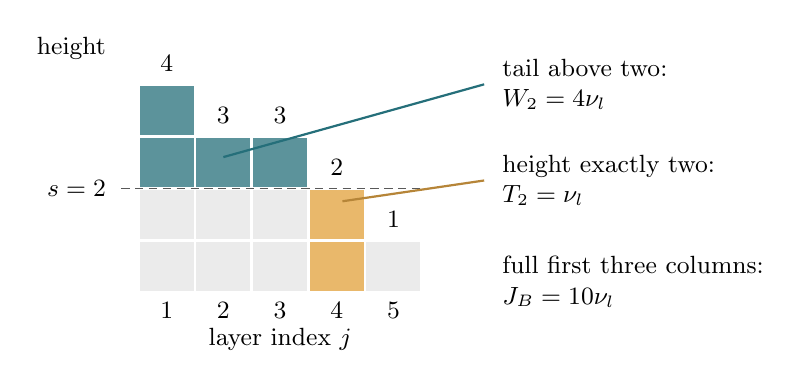
\begin{tikzpicture}[x=0.72cm,y=0.66cm,font=\small]
 \definecolor{layertail}{RGB}{37,111,122}
 \definecolor{layertwo}{RGB}{227,166,70}
 \foreach \j/\height in {1/4,2/3,3/3,4/2,5/1} {
  \foreach \i in {1,...,\height} {
   \fill[black!8] (\j-1,\i-1) rectangle (\j,\i);
   \ifnum\i>2
    \fill[layertail!75] (\j-1,\i-1) rectangle (\j,\i);
   \fi
   \ifnum\j=4
    \fill[layertwo!80] (\j-1,\i-1) rectangle (\j,\i);
   \fi
   \draw[white,line width=1pt] (\j-1,\i-1) rectangle (\j,\i);
  }
  \node[below] at (\j-0.5,0) {\(\j\)};
  \node[above] at (\j-0.5,\height+0.05) {\(\height\)};
 }
 \draw[densely dashed,black!65] (-0.3,2)--(5.3,2);
 \node[anchor=east] at (-0.4,2) {\(s=2\)};
 \node[anchor=east] at (-0.4,4.7) {height};
 \node at (2.5,-0.9) {layer index \(j\)};
 \draw[layertail,thick] (1.5,2.6)--(6.1,4.0);
 \node[anchor=west,align=left] at (6.25,4.0)
   {tail above two:\\ \(W_2=4\nu_l\)};
 \draw[layertwo!80!black,thick] (3.6,1.75)--(6.1,2.15);
 \node[anchor=west,align=left] at (6.25,2.15)
   {height exactly two:\\ \(T_2=\nu_l\)};
 \node[anchor=west,align=left] at (6.25,0.2)
   {full first three columns:\\ \(J_B=10\nu_l\)};
\end{tikzpicture}

 \caption{Layers for a primary group with cyclic exponents
 \((5,4,3,1)\). The column heights are \((4,3,3,2,1)\).
 \(W_2\) and \(J_B\) count selected squares, each of weight
 \(\nu_l\), while \(T_2\) counts each height-two column once.
 The four dark squares above the
 dashed cutoff contribute \(4\nu_l\) to \(W_2\). The orange column
 is the unique layer of height exactly two, contributing \(\nu_l\)
 to \(T_2\). The first three columns have total weight \(10\nu_l\)
 and contribute that amount to \(J_B\).}
 \label{fig:layers}
\end{figure}

We use the slowly varying scales
\begin{equation}\label{eq:layer-scales}
 R=\lceil\ell^2\rceil,
 \qquad \sigma=R^{-6}.
\end{equation}
They will also be used in Section~\ref{sec:paths}.

\begin{proposition}[Static column estimate]\label{prop:static-column}
For every fixed \(L_0\ge1\) and \(e_0>0\), there is a fixed
\(\zeta>0\) such that, typically for nonsingular bit matrices
\(B\) of size \(m\in\mathcal I_N\),
\[
 W_2(B)\le\zeta
 \quad\Longrightarrow\quad
 |\mathcal S_{L_0}(B)|\le2^{e_0N}.
\]
\end{proposition}

The proposition leaves matrices with large \(W_2\) for the path
argument. Its proof separates according to \(T_2\). Layers of height
exactly two can force admissible columns into a few subgroups of large
index; Theorem~\ref{thm:small-intersection} then applies. Otherwise
a coloring controls the pairing on differences of columns. An
arithmetic determinant bound and the spectrum of \(B\) then bound
the dimension of a large subset of one color. We first develop the
pairing argument that distinguishes these two cases.

\subsection{Colors and subgroups of large index}

The \emph{discriminant pairing} of \(B\) is
\begin{equation}\label{eq:discriminant-pairing}
 \lambda_B(\bar x,\bar y)
   =x^{\mathsf T}B^{-1}y\bmod\Z,
 \qquad \bar x,\bar y\in G_B.
\end{equation}
It is well defined because changing either representative by an
integer column combination of \(B\) changes the value by an integer.
It is \emph{perfect}: the map
\(G_B\to\operatorname{Hom}(G_B,\Q/\Z)\) defined by the pairing
is an isomorphism. To see injectivity, an element pairing to zero
with every coordinate class satisfies \(B^{-1}x\in\Z^m\), so its
class is zero; the two finite groups have equal order.
Distinct primary components are orthogonal, since their mutual
pairing is annihilated by coprime powers. An element is called
\emph{isotropic} if its self-pairing is zero. Every
\(z\in\mathcal S_{L_0}(B)\) has isotropic class, and its primary
components are individually isotropic by uniqueness of primary
decomposition in \(\Q/\Z\).

The orthogonal block decomposition of a perfect primary pairing
uses cyclic blocks and, at \(l=2\), possible two-generator blocks
with equal cyclic exponents. These decompositions are classical;
see Miranda~\cite[Section~1]{Miranda}. We use the following precise
consequences of the decomposition and the coloring analysis in
\cite[Lemmas 6.1--6.3]{SymmetricRate}.

\begin{lemma}[Coloring input]\label{lem:pairing-colors}
Let \(B\) be a nonsingular symmetric integer matrix. For each prime
\(l\), put \(f_l=b_{l,3}\). The perfect pairing on \(G_{B,l}\)
admits an orthogonal decomposition
\[
 G_{B,l}=U_l\oplus V_l,
\]
where \(U_l\) consists of the blocks with cyclic exponents strictly
greater than \(f_l\), and the exponent of \(V_l\) divides
\(l^{f_l}\). There are at most two cyclic factors in \(U_l\).
The isotropic elements of \(G_{B,l}\) can be colored with \(C_l\)
colors satisfying
\begin{equation}\label{eq:primary-color-count}
 C_l\le1+8b_{l,1},
 \qquad C_l\le2^{b_{l,2}-b_{l,3}}\quad\text{if \(l\) is odd},
\end{equation}
such that two elements of one color satisfy
\begin{equation}\label{eq:primary-color-pairing}
 l^{f_l}\lambda_B(x_{U_l},y_{U_l})=0
 \quad\text{in }\Q/\Z.
\end{equation}
If \(X\subset G_B\) consists of isotropic elements with one fixed
color at every prime, put \(H=\langle x-y:x,y\in X\rangle\).
Then the image of the \emph{restricted} pairing map
\begin{equation}\label{eq:restricted-pairing-map}
 H\longrightarrow\operatorname{Hom}(H,\Q/\Z),
 \qquad u\longmapsto\lambda_B(u,\cdot)|_H,
\end{equation}
has order at most \(N^{NJ_B}\).
\end{lemma}

The cutoff in Lemma~\ref{lem:pairing-colors} does not split a
block, since the two exponents in each two-generator block are equal.
The restriction in
Equation~\eqref{eq:restricted-pairing-map} is essential: the
characters are tested on \(H\), not on all of \(G_B\).

For our purposes the same coloring has another consequence.

\begin{lemma}[A subgroup containing each color]\label{lem:color-subgroup}
For every prime \(l\), each primary color in
Lemma~\ref{lem:pairing-colors} is contained in a subgroup of
\(G_{B,l}\) whose index is at least
\(l^{b_{l,2}-b_{l,3}}\).
\end{lemma}

\begin{proof}
Write \(f=f_l\) and \(U=U_l\). Multiply the perfect pairing on
\(U\) by \(l^f\), and quotient \(U\) by the radical of this
new pairing. The resulting pairing on a group \(\bar U\) is
perfect. Its order is
\[
 |\bar U|=l^{\sum_i(b_{l,i}-f)_+}.
\]
Indeed, under the original perfect pairing the new radical is
\(U[l^f]=\{u\in U:l^fu=0\}\), and each cyclic factor of exponent
\(b>f\) leaves a quotient of order \(l^{b-f}\).
By Equation~\eqref{eq:primary-color-pairing}, the images of one
color generate a subgroup \(A\subset\bar U\) with
\(A\subset A^\perp\). Perfectness gives
\(|A|\,|A^\perp|=|\bar U|\), so
\[
 [\bar U:A]\ge|\bar U|^{1/2}
 =l^{\frac12\sum_i(b_{l,i}-f)_+}
 \ge l^{b_{l,2}-f}.
\]
Take the preimage of \(A\) in \(U\), and add the unrestricted
summand \(V_l\). This subgroup contains the entire primary color
and has the required index. The argument also covers \(U=0\),
when the asserted index is one.
\end{proof}

The next counting step controls the price of specifying colors. It
uses both bounds in Equation~\eqref{eq:primary-color-count}: the
odd-prime bound is efficient before a weight threshold is reached,
and the polynomial bound controls the prime that crosses it.

\begin{lemma}[Cost of specifying colors]\label{lem:color-cost}
Uniformly over nonsingular symmetric bit matrices of size at most
\(N\), the following hold as \(N\to\infty\).
\begin{enumerate}[label=\textup{(\roman*)}]
 \item If \(T_2(B)\ge\sigma\), there is a set of primes
 \(\mathcal P\) such that
 \[
  \sum_{l\in\mathcal P}(b_{l,2}-b_{l,3})\nu_l\ge\sigma,
  \qquad \sum_{l\in\mathcal P}\log_2 C_l=o(N).
 \]
 \item If \(T_2(B)<\sigma\), then
 \(\sum_l\log_2 C_l=o(N)\).
\end{enumerate}
\end{lemma}

\begin{proof}
The group-order bound gives
\(b_{l,1}\le(N/2)\log_2N\), so the first bound in
Equation~\eqref{eq:primary-color-count} costs \(O(\log N)\) bits
per prime. All primes \(l\le\sqrt N\) together therefore cost
\(O(\sqrt N\log N)=o(N)\).
For larger primes, \(\nu_l>1/(2N)\); they are odd for large
\(N\), and hence
\begin{equation}\label{eq:large-prime-color-cost}
 \sum_{l\in\mathcal P,\ l>\sqrt N}\log_2 C_l
 \le\sum_{l\in\mathcal P,\ l>\sqrt N}(b_{l,2}-b_{l,3})
 \le2N\sum_{l\in\mathcal P,\ l>\sqrt N}
                 (b_{l,2}-b_{l,3})\nu_l.
\end{equation}
For \textup{(i)}, first include every contributing prime at most
\(\sqrt N\). If their total weight is below \(\sigma\), add
larger contributing primes until that threshold is first reached.
Before the last prime, Equation~\eqref{eq:large-prime-color-cost}
costs at most \(2\sigma N\) bits. Charge the last prime only
\(O(\log N)\) bits using the first color bound, regardless of
its weight. The total is \(o(N)\), since \(\sigma\to0\).
For \textup{(ii)}, Equation~\eqref{eq:large-prime-color-cost}
applies to all large primes with total cost at most
\(2\sigma N\); the small-prime cost is unchanged.
\end{proof}

Fix \(0<\alpha<\min\{e_0,1\}\), and impose the typical event of
Theorem~\ref{thm:small-intersection} with \(D=20\). Since
\(\tau=\ell^{-20}=o(\sigma)\), the preceding lemmas settle all
matrices with \(T_2(B)\ge\sigma\). In fact, specify colors only
at the primes selected in Lemma~\ref{lem:color-cost}\textup{(i)}.
There are \(2^{o(N)}\) resulting parts of
\(\mathcal S_{L_0}(B)\). By Lemma~\ref{lem:color-subgroup}, each
part lies in the preimage \(K\subset\Z^m\) of a subgroup of
\(G_B\) with
\[
 B\Z^m\subset K\subset\Z^m,
 \qquad [\Z^m:K]\ge N^{\sigma N}\ge N^{\tau N}.
\]
Theorem~\ref{thm:small-intersection} bounds its size by
\(2^{\alpha N}\). Consequently
\begin{equation}\label{eq:height-two-columns}
 |\mathcal S_{L_0}(B)|\le2^{\alpha N+o(N)}\le2^{e_0N}
\end{equation}
for sufficiently large \(N\). This argument uses the theorem's
simultaneity over all lattices: the color subgroups may depend on
\(B\).

\subsection{A lattice of graph differences}

It remains to control the column set when \(T_2(B)<\sigma\).
The color cost is then subexponential. We first show how two
real-matrix estimates would bound the dimension of a large part of
one color; their probabilistic proofs will follow the comparison.

A nonempty finite set \(\mathcal A\) is \emph{\(\rho\)-robust}
on its affine span \(F\) if every affine subspace \(E\subset F\)
of codimension \(t\) satisfies
\[
 |\mathcal A\cap E|\le2^{-\rho t}|\mathcal A|.
\]
We use the following two geometric inputs from
\cite[Lemmas 3.7 and 3.8]{SymmetricRate}.

\begin{lemma}[Robust extraction]\label{lem:robust-extraction}
If \(\varnothing\ne\mathcal A\subset\bits^m\) and \(\rho>0\),
there is an affine subspace \(E\) for which the nonempty set
\(\mathcal V=\mathcal A\cap E\) is \(\rho\)-robust on its affine
span and satisfies
\[
 \log_2|\mathcal V|\ge\log_2|\mathcal A|-\rho m.
\]
\end{lemma}

\begin{lemma}[Determinant of a robust image lattice]\label{lem:robust-image}
Fix \(D,C_0>0\) and put \(\rho=\ell^{-D}\). Let
\(\varnothing\ne\mathcal V\subset\bits^m\), \(m\le N\), be
\(\rho\)-robust on its affine span \(F\), of dimension \(r\).
Let \(\Phi:F\to\R^d\) be an injective rational affine map such that
\[
 \lVert\Phi(v)-\Phi(w)\rVert_2\le C_0\sqrt N
 \qquad(v,w\in\mathcal V).
\]
Then the integer span of its image differences is a rank-\(r\)
lattice of covolume at most \(\exp(O_{D,C_0}(N\ell))\).
Also
\(H(\Span(\mathcal V-\mathcal V))\le\exp(O_D(N\ell))\).
The covolumes in rank zero are one.
\end{lemma}

For a symmetric matrix \(C\) and a linear subspace
\(F\subseteq\R^m\), the notation \(C|_F\) denotes the
restriction of its bilinear form to \(F\times F\), rather than the
restriction of the associated linear map. Its radical is
\[
 \rad(C|_F)=\{x\in F:x^{\mathsf T}Cy=0\text{ for every }y\in F\}.
\]
Its dimension is the nullity \(\dim F-\rank(C|_F)\).

We will also use a determinant consequence of a finite pairing
image. We include its short proof to make clear why the image order
enters to the first power; this is
\cite[Lemma 6.4]{SymmetricRate}.

\begin{lemma}[Pairing image and determinant]\label{lem:pairing-determinant}
Let \(L\) be a lattice spanning a Euclidean space \(V\), and let
\(q\) be a symmetric bilinear form with \(q(L,L)\subset\Q\).
Set
\[
 K=L\cap\rad q,
 \qquad S=V\cap(\rad q)^\perp.
\]
If the image of \(L\to\operatorname{Hom}(L,\Q/\Z)\),
\(x\mapsto q(x,\cdot)\bmod\Z\), has order \(t\), then
\begin{equation}\label{eq:pairing-det}
 |\det_{\mathrm{orth}}(q|_S)|
 \ge\frac{(\det K)^2}{t(\det L)^2}.
\end{equation}
The determinant on the left is in an orthonormal basis of \(S\).
\end{lemma}

\begin{proof}
The matrix of \(q\) in a lattice basis is rational. Its radical
therefore has a rational basis, so \(K\) spans the radical and is
primitive in \(L\). The orthogonal projection \(\bar L\) of
\(L\) onto \(S\) is a lattice, and
\(\det L=\det K\det\bar L\). The form descends to \(\bar L\)
with the same pairing image order, because pullback of characters
along \(L\to\bar L\) is injective.

Let \(M\) be the nonsingular matrix of the descended form in a
basis of \(\bar L\). Its pairing kernel modulo \(\Z\) in the
coordinate lattice has index \(t\). If \(A\) is an integer basis
matrix for that kernel, then \(|\det A|=t\) and
\(A^{\mathsf T}M\) is integral and nonsingular. Thus
\[
 1\le|\det(A^{\mathsf T}M)|=t|\det M|.
\]
Changing from the lattice basis to an orthonormal basis divides
this determinant by \((\det\bar L)^2\), which proves
Equation~\eqref{eq:pairing-det}. If \(S\) has dimension zero, then \(K=L\) and \(t=1\),
so both sides of Equation~\eqref{eq:pairing-det} are one.
\end{proof}


\begin{lemma}[The graph comparison]\label{lem:graph-comparison}
Fix \(L_0\ge1\) and \(\xi,w>0\). Suppose that \(B\) is a
nonsingular symmetric bit matrix of size \(m\in\mathcal I_N\),
with \(T_2(B)<\sigma\), and that the following hold:
\begin{enumerate}[label=\textup{(\roman*)}]
 \item for every rational \(F\subseteq\R^m\) of height at most
 \(\exp(N\ell^2)\),
 \(\rank(B^{-1}|_F)\ge\dim F-\xi N\);
 \item at most \(\xi N\) eigenvalues of \(B\) lie in
 \([-w\sqrt N,w\sqrt N]\).
\end{enumerate}
Then
\[
 |\mathcal S_{L_0}(B)|\le 2^{(2J_B+2\xi+o(1))N},
\]
where the error tends to zero uniformly over these matrices, for
fixed \(L_0,\xi,w\).
\end{lemma}

\begin{proof}
The assertion is immediate if \(\mathcal S_{L_0}(B)\) is empty.
Choose a largest overall color \(\mathcal A\) of the column set,
and apply Lemma~\ref{lem:robust-extraction} with
\(\rho=\ell^{-2}\). For the resulting set \(\mathcal V\),
Lemma~\ref{lem:color-cost}\textup{(ii)} gives
\begin{equation}\label{eq:robust-column-size}
 \log_2|\mathcal S_{L_0}(B)|
 \le\log_2|\mathcal V|+o(N).
\end{equation}
Put \(F_0=\Span(\mathcal V-\mathcal V)\) and
\(r_0=\dim F_0\). We place each column beside its inverse
image: the norm condition keeps differences short, while the first
coordinates remain integral. The induced graph metric will also
control the inverse form near small eigenvalues of \(B\). Define
the rational graph map and its difference lattice
\[
 \gamma(x)=(x,B^{-1}x),\qquad
 L=\langle\gamma(v)-\gamma(v'):v,v'\in\mathcal V\rangle_{\Z}
       \subset\gamma(F_0).
\]
The graph differences satisfy
\[
 \lVert\gamma(v)-\gamma(v')\rVert_2^2
 \le m+4L_0^2N\le(1+4L_0^2)N.
\]
Lemma~\ref{lem:robust-image}, applied both to the graph map and
to the identity map, consequently gives
\begin{equation}\label{eq:graph-height}
 \det L\le\exp(O_{L_0}(N\ell)),
 \qquad H(F_0)\le\exp(O(N\ell))\le\exp(N\ell^2)
\end{equation}
for sufficiently large \(N\).

On the full graph \(\Gamma=\gamma(\R^m)\), define the rational
symmetric form
\[
 q(\gamma(x),\gamma(y))=x^{\mathsf T}B^{-1}y.
\]
Its restriction to \(\gamma(F_0)\) has rank \(s\) satisfying
\begin{equation}\label{eq:graph-rank}
 s\ge r_0-\xi N
\end{equation}
by the first hypothesis and Equation~\eqref{eq:graph-height}.
The hypothesis covers every subspace of this height, including
\(F_0\), which was selected from admissible columns for \(B\).

The map \(L\to G_B\) taking \(\gamma(u)\) to \(u+B\Z^m\)
has image
\[
 H=\langle\bar v-\bar v':v,v'\in\mathcal V\rangle.
\]
It is surjective onto \(H\), and the form modulo \(\Z\) is the
pullback of the restricted pairing on \(H\). Pullback of characters
is injective, so the two pairing maps have equal image orders.
Lemma~\ref{lem:pairing-colors} bounds this order by \(N^{NJ_B}\).
Let \(K\) be the radical lattice of the restriction to
\(\gamma(F_0)\), and let \(S\) be its radical's orthogonal
complement in that space. The first-coordinate projection is
injective on \(\Gamma\) and takes \(K\) to an integer lattice
of the same rank. Such a lattice has covolume at least one, and
orthogonal projection contracts volumes. Hence \(\det K\ge1\).
Lemma~\ref{lem:pairing-determinant} now yields
\begin{equation}\label{eq:graph-det-lower}
 |\det_{\mathrm{orth}}(q|_S)|
 \ge N^{-NJ_B}\exp(-O_{L_0}(N\ell)).
\end{equation}

The same determinant admits an upper bound from the spectrum of
\(B\). If \(v\) is a unit eigenvector with nonzero eigenvalue
\(x\), its graph vector has squared norm \(1+x^{-2}\), while
\(q(\gamma(v),\gamma(v))=x^{-1}\). Orthogonal eigenvectors of
\(B\) have orthogonal graph vectors. Thus the eigenvalues of the
self-adjoint operator representing \(q\) on \(\Gamma\) are
\[
 \frac{x}{1+x^2}.
\]
They have absolute value at most one. By the second hypothesis,
all but at most \(\xi N\) of them have absolute value at most
\(C_w/\sqrt N\), where \(C_w=1/w\).

The absolute determinant of the compression of a self-adjoint
operator to any \(s\)-dimensional subspace is at most the product
of its largest \(s\) singular values. Indeed, it is
\(\langle\omega,(\bigwedge^s T)\omega\rangle\), where \(\omega\) is the
unit exterior product of an orthonormal basis of the subspace.
Applying this to \(S\), whose dimension is \(s\), gives
\begin{equation}\label{eq:graph-det-upper}
 |\det_{\mathrm{orth}}(q|_S)|
 \le\left(\frac{C_w}{\sqrt N}\right)^{(s-\xi N)_+}.
\end{equation}
This argument applies to indefinite forms and includes \(s=0\).
Combining Equations~\eqref{eq:graph-det-lower}
and~\eqref{eq:graph-det-upper}, and then using
Equation~\eqref{eq:graph-rank}, gives
\[
 (s-\xi N)_+
   \left(\frac12\log N-\log C_w\right)
 \le NJ_B\log N+O_{L_0}(N\ell),
 \qquad
 \frac{r_0}{N}\le2J_B+2\xi+o(1).
\]
The second bound also holds when \(s<\xi N\).

Finally, projection to \(r_0\) suitable coordinates is injective
on the affine span of \(\mathcal V\), so
\(|\mathcal V|\le2^{r_0}\). Equation~\eqref{eq:robust-column-size} and the preceding
dimension bound imply
\[
 \frac1N\log_2|\mathcal S_{L_0}(B)|
 \le 2J_B+2\xi+o(1).
\]
The error is bounded by
\(O_{L_0,w}(\ell^{-2}+\sigma+N^{-1/2}\log N+\ell/\log N)\).
The first three terms come from extraction and colors, and the last
from the determinant comparison, using \(J_B\le1/2\). This
establishes the asserted uniformity.
\end{proof}

\subsection{Uniform rank and spectral estimates}

Lemma~\ref{lem:graph-comparison} identifies the two remaining
probabilistic requirements: inverse forms must retain rank on every
low-height span, and most eigenvalues must stay away from zero at
scale \(\sqrt N\). We now verify both requirements for the biased
bit model. The arguments adapt
\cite[Corollary~5.2 and Proposition~5.4]{SymmetricRate} to the biased
arrays. The rank estimate uses the atom bound \(b\); the spectral
estimate uses the common variance \(pb\) and the rank-two bound
on the mean.

\subsubsection{Inverse forms on low-height subspaces}

\begin{proposition}[Uniform inverse restriction rank]
\label{prop:inverse-rank}
For every fixed \(D>0\) and \(\xi>0\), typically every nonsingular bit
matrix \(B\) satisfies, simultaneously for all rational subspaces
\(F\subseteq\R^m\) with \(H(F)\le\exp(N\ell^D)\),
\[
 \rank(B^{-1}|_F)\ge\dim F-\xi N.
\]
\end{proposition}

\begin{proof}
First fix an arbitrary real subspace \(U\subseteq\R^m\) of dimension
\(d\). Choose a basis matrix \(V\) and a coordinate set \(I\) of size
\(d\) so that \(V_I\) is the identity matrix. Conditional on all
entries of \(B\) outside the principal block \(I\times I\), the
matrix of \(B|_U\) in this basis is
\[
 V^{\mathsf T}BV=B_{I,I}+H,
\]
where \(H\) is a fixed symmetric matrix. The unrevealed entries of
\(B_{I,I}\) are independent bits, each with largest atom \(b\).
Equation~\eqref{eq:typical-corank-tail} therefore shows that
\begin{equation}\label{eq:fixed-restriction-tail}
 \Prob\bigl(\dim\rad(B|_U)\ge\lceil\xi N/2\rceil\bigr)
 \le 2^{-c_{p,\xi}N^2}
\end{equation}
for all sufficiently large \(N\); the event is empty if
\(d<\lceil\xi N/2\rceil\).

For a fixed symmetric form, restricted nullity changes by at most
\(d(U,V)\) when \(U\) is replaced by \(V\). To check this, if
\(Z\subseteq U\) has codimension \(t\), restriction deletes \(t\)
rows and \(t\) columns of a representing matrix. The rank decreases by
an amount between zero and \(2t\), so the nullity changes by at most
\(t\). Apply this first to \(Z=U\cap V\) inside \(U\), then inside
\(V\).

Apply Theorem~\ref{thm:height-cover} with the given \(D\) and any fixed
\(P>0\). Use Equation~\eqref{eq:fixed-restriction-tail} for the
orthogonal complement of every member of its list. The union of all
failures has probability at most
\[
 2^{N^2\ell^{-P}-c_{p,\xi}N^2}=2^{-\Omega_{p,\xi}(N^2)}.
\]
Outside this event, approximate a given \(F\) by a list member. The
nullity comparison and preservation of distance under orthocomplements
give
\[
 \dim\rad(B|_{F^\perp})
 <\lceil\xi N/2\rceil+N\ell^{-P}\le\xi N
\]
for large \(N\). For nonsingular \(B\), the two radicals satisfy
\[
 \rad(B|_{F^\perp})=F^\perp\cap B^{-1}F,
 \qquad
 \rad(B^{-1}|_F)=F\cap B(F^\perp).
\]
Multiplication by \(B\) is an isomorphism from the first space onto
the second. Their equal dimensions prove the proposition.
\end{proof}

\subsubsection{Few eigenvalues near zero}

The preceding argument controls exact nullity on many subspaces. We
also need a metric statement: only a small fraction of the eigenvalues
can be much smaller than \(\sqrt N\). The rank assumption on the mean
enters precisely here.

\begin{proposition}[Small-spectrum bound]\label{prop:small-spectrum}
For every fixed \(\xi>0\), there is \(w_\xi>0\), depending also on
\(p\), such that typically a bit matrix \(B\) has at most \(\xi N\)
eigenvalues, counted with multiplicity, in
\[
 [-w_\xi\sqrt N,w_\xi\sqrt N].
\]
Nonsingularity is not required. The exceptional probability is at most
\(\exp(-c_{p,\xi}N^2)\).
\end{proposition}

\begin{proof}
Set
\[
 X=\frac{B-\E B}{\sqrt{mpb}},\qquad
 \mu_X=\frac1m\sum_{i=1}^m\delta_{\lambda_i(X)}.
\]
We first verify that the expected measures \(\E\mu_X\) converge
uniformly over the permitted arrays to the semicircle law
\[
 d\mu_{\mathrm{sc}}(x)=\frac1{2\pi}\sqrt{4-x^2}\,
                       \ind{|x|\le2}\,dx.
\]
This is the fixed-moment argument for Wigner's law~\cite{Wigner}.
The centered, variance-standardized entries
\((B_{ij}-\E B_{ij})/\sqrt{pb}\) have mean zero, variance one, and
uniformly bounded moments of every fixed order. Expand
\(m^{-1}\E\operatorname{Tr}X^s\) as a sum over closed walks of length
\(s\). Independence makes a summand zero whenever an unordered edge
is used exactly once. Every remaining walk has at most \(s/2\)
distinct edges and at most \(1+s/2\) vertices. For each fixed walk
pattern with \(v<1+s/2\) vertices, its contribution is
\(O_{p,s}(m^{v-1-s/2})=o(1)\). Equality is possible only when \(s\)
is even and the walk traverses each edge of a tree twice. Each such
pattern contributes \(1+o(1)\), since it uses only variances, and
there are \((s/2+1)^{-1}\binom{s}{s/2}\) patterns. There are finitely
many patterns for fixed \(s\), so the errors are uniform. The limiting
moments are those of \(\mu_{\mathrm{sc}}\); its compact support makes
them determinate. The method of moments proves the asserted weak
convergence, uniformly by applying the same argument to any sequence of
permitted arrays.

Choose a fixed \(w>0\), sufficiently small in terms of \(\xi\), and
put
\[
 f(x)=(1-|x|/w)_+.
\]
The semicircle mass of \([-w,w]\) tends to zero with \(w\), so the
convergence just proved gives, for sufficiently large \(N\),
\begin{equation}\label{eq:typical-tent-mean}
 \E\operatorname{Tr}f(X)\le\xi m/16.
\end{equation}
To obtain a much stronger probability estimate than moment convergence
alone provides, write
\[
 f=1-g_1+g_2,\qquad
 g_1(x)=|x|/w,\quad g_2(x)=(|x|/w-1)_+.
\]
Both functions are convex and \(1/w\)-Lipschitz, and their matrix
traces are convex functions of the entries. If \(M_+\) denotes the
spectral positive part of \(M\), then
\(\operatorname{Tr}M_+=\sup_{0\preceq P\preceq I}\operatorname{Tr}(PM)\)
for symmetric \(M\); expressing the two traces as sums of positive-part
traces proves convexity directly.

Let \(y\) denote the independent upper-triangular coordinates, and
write \(X(y)\) for the corresponding centered, normalized matrix.
The Hoffman--Wielandt inequality~\cite[Theorem~1]{HoffmanWielandt}
and Cauchy--Schwarz give, for \(j=1,2\),
\[
 \left|\operatorname{Tr}g_j(X(y))-
             \operatorname{Tr}g_j(X(y'))\right|
 \le\frac{\sqrt m}{w}\lVert X(y)-X(y')\rVert_F
 \le\frac1w\sqrt{\frac2{pb}}\lVert y-y'\rVert_2.
\]
Here \(\lVert\cdot\rVert_F\) is the Frobenius norm, and the factor
\(2\) accounts for reflecting off-diagonal entries. The convex Lipschitz
consequence of Talagrand's convex-distance inequality
\cite[Theorem~4.1.1]{Talagrand} applies to independent coordinates in
\([0,1]\) with arbitrary distributions: if \(F\) is
convex and \(L\)-Lipschitz, then
\[
 \Prob(|F-\E F|>t)\le C\exp(-ct^2/L^2).
\]
The usual median formulation implies this expectation formulation by
integrating the tail and adjusting the absolute constants. Applying it
to the two convex traces, with deviations \(\xi m/32\), and using
Equation~\eqref{eq:typical-tent-mean}, gives
\[
 \Prob\bigl(\operatorname{Tr}f(X)>\xi m/8\bigr)
 \le C\exp(-c_{p,\xi,w}m^2).
\]
On the complementary event, \(f\ge1/2\) on \([-w/2,w/2]\) implies
that at most \(\xi m/4\) eigenvalues of \(X\) lie in this interval.
The matrix \(B/\sqrt{mpb}\) differs from \(X\) by a matrix of rank
at most two. Interlacing changes the count in any interval by at most
four. Taking, for example, \(w_\xi=w\sqrt{pb}/4\), we have
\(w_\xi\sqrt{N/(mpb)}\le w/2\) for large \(N\), uniformly in
\(m\in\mathcal I_N\). The requested eigenvalue count is therefore
at most \(\xi m/4+4\le\xi N\).
\end{proof}


\begin{proof}[Proof of Proposition~\ref{prop:static-column}]
Fix \(L_0\ge1\) and \(e_0>0\). Choose fixed \(\xi,\zeta>0\)
with \(6\zeta+2\xi<e_0\). Intersect the typical event used for
Equation~\eqref{eq:height-two-columns} with the events in
Propositions~\ref{prop:inverse-rank} and~\ref{prop:small-spectrum},
taking height exponent \(D=2\) and error \(\xi\). The latter
proposition supplies a fixed \(w_\xi>0\). This finite intersection
is still typical, uniformly in the permitted models and sizes.

Let \(B\) be nonsingular on this event, with \(W_2(B)\le\zeta\).
If \(T_2(B)\ge\sigma\), Equation~\eqref{eq:height-two-columns}
already gives the required bound. Otherwise apply
Lemma~\ref{lem:graph-comparison} with \(w=w_\xi\).
Equation~\eqref{eq:pairing-high-tail} gives
\[
 |\mathcal S_{L_0}(B)|
 \le2^{(2J_B+2\xi+o(1))N}
 \le2^{(6\zeta+2\xi+o(1))N}
 \le2^{e_0N}
\]
for all sufficiently large \(N\). This proves the proposition.
\end{proof}

\section{Two column constraints along a path of principal minors}\label{sec:paths}

Proposition~\ref{prop:static-column} bounds the admissible columns when
\(W_2\) is small. We now show that a terminal matrix with large \(W_2\)
must encounter two rare column constraints along a short path of principal
minors. Each constraint costs almost \(b^N\), giving the exceptional
probability required in Proposition~\ref{prop:column-bound}.
The principal-minor method and its layer recursion come from
\cite[Sections 7 and 11]{SymmetricRate}. We first state the deterministic
inputs, then give the probability estimates for biased columns.

\subsection{Principal extensions and retained layers}

A principal extension of width \(h\in\{1,2\}\) has the form
\begin{equation}\label{eq:path-extension}
 B=\begin{pmatrix}C&V\\V^{\mathsf T}&D\end{pmatrix},
 \qquad V=(v_1\ \cdots\ v_h),
\end{equation}
where \(C\) is nonsingular and \(D\) is symmetric. At width two we impose
the \emph{gate}
\begin{equation}\label{eq:path-gate}
 v_1,v_2\in\mathcal S_{L_0}(C).
\end{equation}
There is no gate at width one. The following elementary fact ensures that
every nonsingular bit matrix can be reached by a path with these gates.

\begin{lemma}[Gated deletion, {\cite[Lemma 7.1]{SymmetricRate}}]
\label{lem:path-deletion}
Let \(B\) be a nonsingular symmetric bit matrix of positive size.
The empty principal minor has determinant one, and its admissible
column set consists of the unique empty column.
Either some one-coordinate principal deletion is nonsingular, or a
two-coordinate principal deletion gives a nonsingular matrix \(C\) for
which both deleted cross columns satisfy
\[
 v_i^{\mathsf T}C^{-1}v_i\in\bits,
 \qquad \lVert C^{-1}v_i\rVert_\infty\le1
 \quad(i=1,2).
\]
In particular, whenever the sizes belong to \(\mathcal I_N\), the
two-coordinate move satisfies Equation~\eqref{eq:path-gate}.
\end{lemma}

\begin{proof}
The cofactor identity gives the first alternative if some diagonal entry
of \(B^{-1}\) is nonzero. Otherwise choose distinct \(i,j\) maximizing
the absolute value of an entry of \(B^{-1}\), and write
\(\kappa=(B^{-1})_{ij}\ne0\). The corresponding principal block is
\(\left(\begin{smallmatrix}0&\kappa\\\kappa&0\end{smallmatrix}\right)\).
Jacobi's complementary minor identity makes the complementary matrix
\(C\) nonsingular. In the block notation of
Equation~\eqref{eq:path-extension}, its Schur complement
\(T=D-V^{\mathsf T}C^{-1}V\) satisfies
\[
 T^{-1}=\begin{pmatrix}0&\kappa\\\kappa&0\end{pmatrix},
 \qquad (B^{-1})_{I,\{i,j\}}=-C^{-1}VT^{-1},
\]
where \(I\) is the set of remaining indices. The diagonal of \(T\)
vanishes, giving the two quadratic identities. The two columns of the
inverse block on the right are \(-\kappa C^{-1}v_2\) and
\(-\kappa C^{-1}v_1\). Their entries have absolute value at most
\(|\kappa|\), proving the norm bound. Finally
\(\lVert C^{-1}v_i\rVert_2\le\sqrt{\operatorname{size}(C)}
\le\sqrt N\le L_0\sqrt N\).
\end{proof}

For an extension with nonsingular start \(C\), define the successive
quotients
\begin{equation}\label{eq:path-quotients}
 G_0=G_C,\qquad
 G_i=\Z^m/(C\Z^m+\Z v_1+\cdots+\Z v_i)
       =G_{i-1}/\langle\overline v_i\rangle
       \quad(1\le i\le h),
\end{equation}
where \(m=\operatorname{size}(C)\). These groups are defined even if
the endpoint \(B\) is singular. In a one-element quotient, each layer
height drops by zero or one. A positive layer whose height does not
drop is called \emph{retained}. A \emph{plateau} is a maximal interval
of consecutive layers of equal positive height at one prime. On each
plateau, the retained layers form a prefix, possibly empty. These
facts are Lemma~7.3 of \cite{SymmetricRate}; for example the prefix
assertion follows because quotient heights are nonincreasing and can
only equal the original height or one less.

Here are the remaining group-theoretic inputs in the precise form
needed below.

\begin{lemma}[Retention lattices and tail recursion]
\label{lem:path-algebra}
Let \(C\) be a nonsingular symmetric bit matrix of size \(m\le N\).
\begin{enumerate}[label=\textnormal{(\roman*)}]
\item Let \(\pi:\Z^m\twoheadrightarrow G\) be a quotient map with
\(C\Z^m\subseteq\ker\pi\). For any set \(\mathcal D\) of positive
layers of \(G\), there is a lattice \(K_{\mathcal D}\), fixed by
\(\pi,G,\mathcal D\), such that
\begin{equation}\label{eq:path-retention-lattice}
 C\Z^m\subseteq K_{\mathcal D}\subseteq\Z^m,
 \qquad [\Z^m:K_{\mathcal D}]=N^{Nq(\mathcal D)},
 \quad q(\mathcal D)=\sum_{(l,j)\in\mathcal D}k_G(l,j)\nu_l.
\end{equation}
If every layer in \(\mathcal D\) is retained on quotienting by
\(\pi(v)\), then \(v\in K_{\mathcal D}\).
\item Suppose the extension in Equation~\eqref{eq:path-extension}
also has nonsingular endpoint \(B\). Then
\(k_B(l,j)\le k_C(l,j)+h\) for every layer. Writing
\(\mathcal R_i\) for the retained layers in \(G_{i-1}\to G_i\),
for every integer \(s\ge h\) we have
\begin{equation}\label{eq:path-tail-recursion}
 W_s(B)\le W_{s+h}(C)
   +2\sum_{i=1}^h
       \sum_{\substack{(l,j)\in\mathcal R_i\\
                        k_{G_{i-1}}(l,j)\ge s+1-h}}\nu_l.
\end{equation}
\end{enumerate}
\end{lemma}

\begin{proof}[Source and interpretation]
Part~\textnormal{(i)} is the Retention lattice lemma
\cite[Lemma 7.4]{SymmetricRate}, including arbitrary, nonconsecutive
sets of layers. Part~\textnormal{(ii)} is the Tail recursion lemma
\cite[Lemma 11.1]{SymmetricRate} together with common-quotient
interlacing \cite[Equation (7.11)]{SymmetricRate}. For the latter,
projection onto the old coordinates identifies \(G_h\) with the
quotient of \(G_B\) by the \(h\) new coordinate classes. Since a
one-element quotient lowers each height by at most one,
\(k_B\le k_{G_h}+h\le k_C+h\).
The stronger recursion uses symmetry through the Symmetric kernel
inequality \cite[Lemma 7.5]{SymmetricRate}; it needs no assumption on
the entry distribution. All of these statements therefore apply to
the present biased model.
\end{proof}

\subsection{The cost of retaining layers}

Fix \(L_0\ge1\), a sufficiently small fixed \(e_0>0\), and the
corresponding \(\zeta>0\) in Proposition~\ref{prop:static-column}.
Recall \(R=\lceil\ell^2\rceil\) and \(\sigma=R^{-6}\).
Call an extension \emph{costly} if, in at least one of its quotient
operations,
\begin{equation}\label{eq:path-costly-definition}
 \sum_{(l,j)\in\mathcal R_i}\nu_l\ge\sigma.
\end{equation}
We use this name only for the condition in
Equation~\eqref{eq:path-costly-definition}.

In all column estimates, the information already exposed fixes the
start \(C\), and possibly a preceding column of the same width-two
extension. The next column has independent bit entries with success
probabilities \(p\) or \(b\). The quotient map is thus fixed before
the next column is tested.

\begin{lemma}[Almost full cost of retention]\label{lem:path-retention-cost}
Typically for nonsingular \(C\) with size in \(\mathcal I_N\),
conditional on \(C\), the probability that an independent principal
extension of either width is costly is at most
\begin{equation}\label{eq:path-retention-cost}
 p_N:=2^{-N(a-2e_0)}.
\end{equation}
For one specified column, the probability that its retained weight
is at least \(\sigma\) obeys the same bound, also after exposing the
preceding column of a width-two extension. Also, typically, when
\(W_2(C)\le\zeta\), the width-two gate has conditional probability
at most \(p_N^2\).
\end{lemma}

\begin{proof}
Impose Theorem~\ref{thm:small-intersection} on \(C\) with
\(\tau=\ell^{-20}\) and some fixed \(0<\alpha<e_0\).
Then \(\tau=o(\sigma)\). We show that the retention condition can be
covered by \(2^{o(N)}\) selected layer sets, each giving a lattice of
index at least \(N^{\sigma N}\).

Let \(G\) be the group before one column is tested. It is a quotient
of \(G_C\), so its total height times weight is at most \(1/2\).
At a prime \(l\), let \(d_l\) be its number of plateaus. Distinct
positive plateau heights give
\(d_l^2\le2\sum_j k_G(l,j)\), and the group-order bound gives
\(\sum_{l,j}k_G(l,j)=O(N\log N)\). Consequently the number of
plateaus at primes \(l\le\sqrt N\) is
\(O(N^{3/4}\sqrt{\log N})\), by Cauchy--Schwarz. Each prefix
length has \(O(N\log N)\) possible values. Thus the complete
retention pattern at these primes can be specified with
\begin{equation}\label{eq:path-small-prime-entropy}
 O\bigl(N^{3/4}(\log N)^{3/2}\bigr)=o(N)
\end{equation}
bits. Include all those retained layers in the selected set.

If their total weight is below \(\sigma\), add retained layers at
primes \(l>\sqrt N\) until the total first reaches \(\sigma\).
There are at most \(N\) candidate layers in this prime range, since
each has \(\nu_l>1/(2N)\). At most
\(\lceil2\sigma N\rceil+1\) additions suffice. The binomial bound
therefore contributes \(2^{o(N)}\) further possibilities. This
constructs the claimed cover whenever the retained weight is at
least \(\sigma\).

For every selected set \(\mathcal D\), positive heights and
Equation~\eqref{eq:path-retention-lattice} give
\(q(\mathcal D)\ge\sigma\). The simultaneous cube estimate applies
to \(K_{\mathcal D}\), since it contains \(C\Z^m\), even when
\(G\) depends on an earlier column. Each cube point has probability
at most \(b^m\), where \(m=N-o(N)\). The one-column probability is
therefore at most
\[
 2^{o(N)}2^{\alpha N}b^m
       =2^{-N(a-\alpha-o(1))}.
\]
The slack \(\alpha<e_0\) absorbs a union over at most two columns
and yields Equation~\eqref{eq:path-retention-cost}.

Finally impose Proposition~\ref{prop:static-column} on the start.
When \(W_2(C)\le\zeta\), each column belongs to
\(\mathcal S_{L_0}(C)\) with probability at most \(2^{e_0N}b^m\).
The two cross columns are independent conditional on \(C\), so the
gate probability is at most
\((2^{e_0N}b^m)^2\le p_N^2\).
\end{proof}

We also need a weaker estimate that applies without typicality. Its
role is to prevent a path from carrying substantial weight in very
high layers. The elementary counting argument below is the biased
version of \cite[Lemma 11.2]{SymmetricRate}.

\begin{lemma}[Dissociation and a lattice constraint]\label{lem:path-dissociation}
Let \(C\) be a nonsingular bit matrix of size \(m\le N\), and let
\(C\Z^m\subseteq K\subseteq\Z^m\) have index \(N^{qN}\).
If \(v\) has independent bit coordinates, each with maximum atom
at most \(b\), then
\begin{equation}\label{eq:path-fixed-mask-cost}
 \Prob(v\in K)\le b^{2qN/3}.
\end{equation}
\end{lemma}

\begin{proof}
Write \(g_1,\ldots,g_m\) for the coordinate images in \(\Z^m/K\).
Choose a maximal set of \(j\) of these images whose subset sums
are all distinct. Such a set is called \emph{dissociated}. Once
the other bits are fixed, at most one assignment of these \(j\)
bits gives zero in the quotient, and that assignment has probability
at most \(b^j\).

Maximality says that every \(g_i\) is a combination of the selected
images with coefficients in \(\{-1,0,1\}\): otherwise adding it
would preserve distinct subset sums. Put these coefficients in a
\(j\)-by-\(m\) integer matrix \(M\), using identity columns at the
selected indices. Then \(\rank M=\rank(MC)=j\), and evaluation
of the selected images is a surjection
\(\theta:\Z^j\twoheadrightarrow\Z^m/K\). Every column of \(MC\)
lies in \(\ker\theta\). Choose \(j\) independent such columns;
each has norm at most \(N\sqrt j\). The index of their integer
span bounds the quotient order, so Hadamard's inequality gives
\[
 N^{qN}\le(N\sqrt j)^j\le N^{3j/2}.
\]
Thus \(j\ge2qN/3\), proving the assertion. If \(j=0\), the
quotient is trivial and the same conclusion holds with empty products.
\end{proof}

For one column with pre-test group \(G\), write
\begin{equation}\label{eq:path-heavy-weight}
 Q_{\rm hi}=\sum_{\substack{(l,j)\text{ retained}\\k_G(l,j)\ge R-1}}
                     k_G(l,j)\nu_l.
\end{equation}

\begin{lemma}[Cost of heavy retained layers]\label{lem:path-heavy-cost}
Fix \(0<\eta<1\), and put \(q_{\min}=\eta/(100\log N)\).
There is a constant \(c_p>0\) such that, uniformly for
\(q_{\min}\le q\le1/2\),
\begin{equation}\label{eq:path-heavy-cost}
 \Prob\bigl(Q_{\rm hi}\in[q,2q)\mid\text{previous exposure}\bigr)
       \le2^{-c_pqN}.
\end{equation}
This holds whenever the previous exposure fixes a nonsingular start
\(C\) of size in \(\mathcal I_N\), and a quotient map to \(G\)
whose kernel contains \(C\Z^m\), while leaving the tested bits
independent with success probabilities \(p\) or \(b\).
\end{lemma}

\begin{proof}
For a fixed set \(\mathcal D\) of retained layers, the retention
lattice and Lemma~\ref{lem:path-dissociation} give cost
\(2^{-(2a/3)q(\mathcal D)N}\). Enumerate the sets consisting of
all retained layers of height at least \(R-1\), with their total
height times weight in \([q,2q)\).

For primes at most \(\sqrt N\), prefix lengths on the eligible
plateaus specify the set. Equation~\eqref{eq:path-small-prime-entropy}
costs
\[
 O\bigl(N^{3/4}(\log N)^{3/2}\bigr)
       =o(N/\log N)=o_\eta(qN)
\]
bits uniformly over the stated range. At larger primes each eligible
layer contributes at least \((R-1)/(2N)\). There are therefore
\(O(N/R)\) eligible layers in total, and a set of weight below
\(2q\) contains at most \(O(qN/R)\) of them. The binomial estimate,
or the all-subsets bound when \(q\) is bounded below, gives logarithmic
count
\[
 O\!\left(\frac{qN}{R}\bigl(1+\log(1/q)\bigr)\right)
       =o_\eta(qN).
\]
Indeed \(1+\log(1/q)=O_\eta(\ell)\), \(R\asymp\ell^2\),
and \(qN/R\to\infty\) uniformly, so rounding has no effect.
Every counted set has \(q(\mathcal D)\ge q\). Its probability
cost absorbs both entropy bounds; for instance any fixed
\(0<c_p<2a/3\) works for all sufficiently large \(N\).
\end{proof}

\subsection{Fixed paths and removal of high layers}

We now turn the column estimates into a bound on terminal matrices.
Let
\[
 H_0=2\lceil N^{3/5}\rceil,\qquad m_*=N-1.
\]
Consider all fixed index paths
\begin{equation}\label{eq:path-index-path}
 I_0\subset I_1\subset\cdots\subset I_{H_0}=[m_*],
 \qquad h_t=|I_t\setminus I_{t-1}|\in\{1,2\}.
\end{equation}
Fix an ordering of each pair of new indices. At a backward step there
are at most \(2N^2\) choices, so the number of paths is at most
\begin{equation}\label{eq:path-count}
 (2N^2)^{H_0}=2^{O(N^{3/5}\log N)}=2^{o(N)}.
\end{equation}
Every node size belongs to \(\mathcal I_N\), since at most
\(2H_0=o(N^{7/10})\) indices are deleted.

Let \(\mathcal T_m\) be the set of nonsingular size-\(m\) matrices
satisfying Lemma~\ref{lem:prime-corank},
Proposition~\ref{prop:static-column}, and the simultaneous cube
property used in Lemma~\ref{lem:path-retention-cost}.
Their exceptional probabilities are uniformly \(2^{-\omega(N)}\).
Every fixed principal submatrix remains in the bit model: its
upper-triangular entries are independent with the prescribed biases,
and its mean is a principal submatrix of the original mean, hence
has rank at most two.
A union bound using Equation~\eqref{eq:path-count} shows that the
probability of any nonsingular node on any path failing these
requirements is still \(2^{-\omega(N)}\).

For one fixed path, write \(B_t=B[I_t]\), and let
\(\mathcal A\) be the event that all its nodes belong to their
respective \(\mathcal T_m\) and every width-two gate holds.
Lemma~\ref{lem:path-deletion}, applied backwards \(H_0\) times,
shows that every nonsingular terminal matrix outside the exceptional
event belongs to \(\mathcal A\) for at least one fixed path.

For the probability estimates, expose a fixed path \emph{forwards}:
first \(B_0\), then the cross columns and new symmetric block of
each extension. Conditional on everything already exposed, a cross
column has independent entries of the original prescribed biases.
The second cross column of a pair remains independent after the first
has been revealed. Future typicality, nonsingularity and gate
requirements enter only through the event \(\mathcal A\).

Call the last \(5R\) steps, together with their \(5R+1\) nodes,
the \emph{terminal window}. We first remove paths with a large
\(W_R\) anywhere in that window.

\begin{lemma}[Small high-layer tails on the window]\label{lem:path-high-tail}
For every fixed \(0<\eta<1\), each fixed path satisfies
\begin{equation}\label{eq:path-high-tail}
 \Prob\!\left(\mathcal A,
       \max_{H_0-5R\le t\le H_0} W_R(B_t)>\eta\right)
       \le2^{-\Omega_{p,\eta}(NR)}.
\end{equation}
\end{lemma}

\begin{proof}
At each tested column form \(Q_{\rm hi}\) from
Equation~\eqref{eq:path-heavy-weight}, and put
\[
 \widetilde Q=
 \begin{cases}
 Q_{\rm hi},&Q_{\rm hi}\ge q_{\min},\\
 0,&Q_{\rm hi}<q_{\min},
 \end{cases}
 \qquad q_{\min}=\frac{\eta}{100\log N}.
\]
Set \(\widetilde Q=0\) for every cross column of a step with singular
start. This defines the quantities on the entire exposure space.
At nonsingular starts, \(Q_{\rm hi}\le1/2\). For dyadic values
\(q_j=2^jq_{\min}\le1/2\), Lemma~\ref{lem:path-heavy-cost} gives,
with any fixed \(0<c'_p<c_p/2\),
\begin{align}
 \E\!\left[2^{c'_pN\widetilde Q}\mid\text{previous exposure}\right]
 &\le 1+\sum_{j:q_j\le1/2}2^{2c'_pNq_j}2^{-c_pNq_j}\notag\\
 &\le1+2^{-\Omega_{p,\eta}(N/\log N)}.
 \label{eq:path-heavy-one-moment}
\end{align}
The same bound holds at singular starts. There are at most \(2H_0\)
tested columns. Successive conditioning, including between columns of
a pair, yields
\begin{equation}\label{eq:path-heavy-total-moment}
 \E\,2^{c'_pN\sum\widetilde Q}\le1+o(1).
\end{equation}

On \(\mathcal A\), suppose a window node has \(W_R>\eta\).
Iterate Equation~\eqref{eq:path-tail-recursion} backwards from that
node, beginning with \(s=R\) and increasing \(s\) by the width at
each step. Stop once \(s>N^{3/5}\). This takes at most
\(\lceil N^{3/5}\rceil\) steps; even the earliest window node has
\(H_0-5R>\lceil N^{3/5}\rceil\) predecessors for large \(N\).
The final tail vanishes because Lemma~\ref{lem:prime-corank} bounds
every layer height by \(N^{3/5}\).

Number these backwards steps by \(j=1,2,\ldots\). At step \(j\),
the threshold in the recursion is \(R\) plus the preceding widths,
so every charged layer has height at least
\[
 s+1-h\ge R+j-2\ge R-1.
\]
The contribution from one column is therefore at most
\(2Q_{\rm hi}/(R+j-2)\). There are at most two columns per step.
All contributions with \(Q_{\rm hi}<q_{\min}\) total at most
\[
 4q_{\min}\sum_j\frac1{R+j-2}
       \le4q_{\min}(1+\log N)<\eta/2.
\]
The remaining contributions must exceed \(\eta/2\). Their
denominators are at least \(R-1\), and consequently
\begin{equation}\label{eq:path-heavy-forced-sum}
 \sum\widetilde Q\ge\frac{(R-1)\eta}{4},
\end{equation}
where the sum may be extended to all tests on the fixed path.
This same necessary condition holds for a violation at any window
node. Markov's inequality and
Equation~\eqref{eq:path-heavy-total-moment} prove the claim.
\end{proof}

\subsection{The terminal window forces two constraints}

Choose a fixed
\(0<\eta<\min\{1,\zeta/4\}\). The preceding lemma leaves only
windows with \(W_R\le\eta\) at every node. On such a window,
the following deterministic argument is the reason that two full
column costs suffice.

\begin{lemma}[The terminal-window alternative]\label{lem:path-window}
Consider \(5R\) consecutive nonsingular principal extensions of
widths one or two, satisfying their gates. Suppose all their nodes
have \(W_R\le\eta\) and the terminal node has \(W_2>\zeta\).
For all sufficiently large \(N\), either at least two distinct steps
are costly, or a width-two step starts at a node with
\(W_2\le\zeta\).
\end{lemma}

\begin{proof}
At a noncostly step of width \(h\), the recursion gives
\begin{equation}\label{eq:path-noncostly}
 W_s(B)\le W_{s+h}(C)+4\sigma
       \qquad(s\ge h).
\end{equation}
Iterate this inequality from \(s=2\) backwards over any block of
\(R\) noncostly steps. The threshold increases by at least \(R\),
so the endpoint satisfies
\[
 W_2\le\delta,\qquad \delta:=\eta+4R\sigma.
\]
Here and below \(\delta<\zeta\) for large \(N\).

Label the window nodes \(X_0,\ldots,X_{5R}\). If there are no
costly steps, the last \(R\) steps contradict the terminal value.
Suppose there is exactly one costly step, at position \(t\).
There must be fewer than \(R\) steps after it, or the same argument
again applies. Thus \(t\ge4R+1\). Both \(X_{t-2}\) and
\(X_{t-1}\) end blocks of \(R\) noncostly steps inside the window,
and hence both have \(W_2\le\delta\).

Assume there is no width-two step whose starting \(W_2\) is at
most \(\zeta\). The two steps at positions \(t-1,t\) must then
both have width one. Applying Equation~\eqref{eq:path-noncostly}
with \(s=1\) to the preceding step gives
\[
 W_1(X_{t-1})\le W_2(X_{t-2})+4\sigma\le\delta+4\sigma.
\]
Even though step \(t\) is costly, its width is one, so the height
comparison in Lemma~\ref{lem:path-algebra} gives
\[
 W_2(X_t)\le W_1(X_{t-1})\le\delta+4\sigma.
\]
The remaining steps are noncostly. For either width,
Equation~\eqref{eq:path-noncostly} with \(s=2\) and monotonicity
of \(W_s\) in \(s\) show that each increases \(W_2\) by at most
\(4\sigma\). There are fewer than \(R\) such steps, whence
\[
 W_2(X_{5R})\le\eta+8R\sigma<\zeta,
\]
a contradiction. Figure~\ref{fig:terminal-window} records the two
adjacent width-one steps used in this argument.
\end{proof}

\begin{figure}[tbp]
\centering
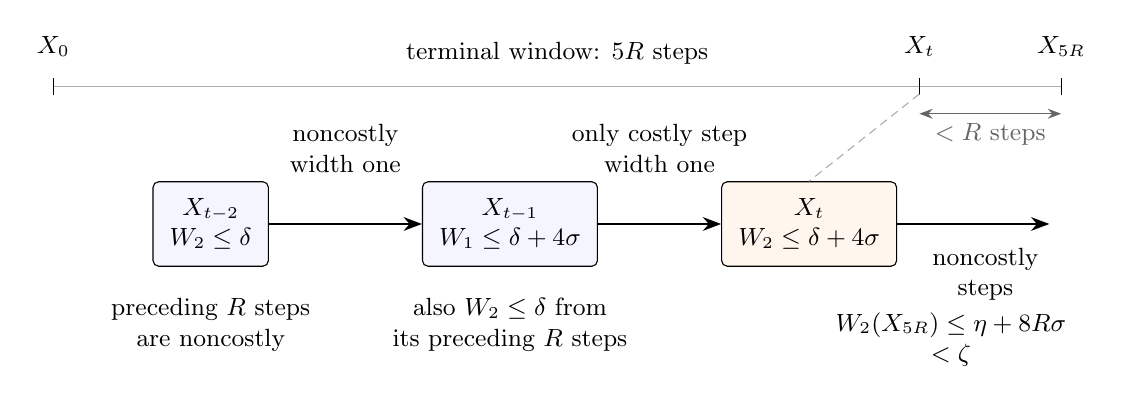
\begin{tikzpicture}[x=1cm,y=1cm,>=Stealth,font=\small]
 \draw[gray!65] (0,1.75)--(12.8,1.75);
 \draw (0,1.64)--(0,1.86) node[above=4pt] {$X_0$};
 \draw (12.8,1.64)--(12.8,1.86) node[above=4pt] {$X_{5R}$};
 \draw (11,1.64)--(11,1.86) node[above=4pt] {$X_t$};
 \node[above] at (6.4,1.9) {terminal window: $5R$ steps};
 \draw[<->,gray!80!black] (11,1.4)--(12.8,1.4)
       node[midway,below] {$<R$ steps};
 \node[draw,rounded corners=2pt,align=center,inner sep=6pt,
       fill=blue!4] (left) at (2.0,0)
       {$X_{t-2}$\\$W_2\le\delta$};
 \node[draw,rounded corners=2pt,align=center,inner sep=6pt,
       fill=blue!4] (middle) at (5.8,0)
       {$X_{t-1}$\\$W_1\le\delta+4\sigma$};
 \node[draw,rounded corners=2pt,align=center,inner sep=6pt,
       fill=orange!7] (right) at (9.6,0)
       {$X_t$\\$W_2\le\delta+4\sigma$};
 \draw[->,thick] (left)--(middle)
       node[midway,above=15pt,align=center] {noncostly\\width one};
 \draw[->,thick] (middle)--(right)
       node[midway,above=15pt,align=center] {only costly step\\width one};
 \draw[densely dashed,gray!65] (11,1.65)--(right.north);
 \node[below=8pt,align=center] at (left.south)
       {preceding $R$ steps\\are noncostly};
 \node[below=8pt,align=center] at (middle.south)
       {also $W_2\le\delta$ from\\its preceding $R$ steps};
 \draw[->,thick] (right.east)--(12.65,0)
       node[pos=.58,below=5pt,align=center] {noncostly\\steps};
 \node[align=center,anchor=north] at (11.4,-1.0)
       {$W_2(X_{5R})\le\eta+8R\sigma$\\$<\zeta$};
\end{tikzpicture}

\caption{The contradiction setup in Lemma~\ref{lem:path-window}:
suppose the window has only one costly step and no width-two step
starts with \(W_2\le\zeta\). The costly step is within \(R\)
steps of the end. Each of its two preceding nodes ends an \(R\)-step
noncostly block, and the displayed adjacent steps must have width
one. The lower chain enlarges these adjacent steps; horizontal
spacing is schematic. The labels are upper bounds propagated by
the proof, not a plot of a matrix statistic.
Here \(\delta=\eta+4R\sigma\).}
\label{fig:terminal-window}
\end{figure}

\begin{proof}[Proof of Proposition~\ref{prop:column-bound}]
Outside a set of probability \(2^{-\omega(N)}\), every nonsingular
terminal matrix belongs to a required fixed-path event \(\mathcal A\).
By Lemma~\ref{lem:path-high-tail} and Equation~\eqref{eq:path-count},
we may also exclude, at the same scale, all such path events having
\(W_R>\eta\) anywhere in their windows.

For a fixed remaining path with terminal \(W_2>\zeta\),
Lemma~\ref{lem:path-window} forces either two costly positions or
a width-two gate with starting \(W_2\le\zeta\). To make the
conditional probability calculation explicit, let \(\mathcal F_t\)
contain all entries exposed through step \(t\). Define \(D_t\)
to be the event that the starting matrix is in its typical set and
step \(t\) is costly. Its starting-matrix indicator is
\(\mathcal F_{t-1}\)-measurable, and
Lemma~\ref{lem:path-retention-cost} gives
\[
 \E[\ind{D_t}\mid\mathcal F_{t-1}]\le p_N.
\]
For any two positions \(r<t\), including consecutive ones,
\begin{equation}\label{eq:path-two-positions}
 \Prob(D_r\cap D_t)
 =\E\!\left[\ind{D_r}
       \E[\ind{D_t}\mid\mathcal F_{t-1}]\right]
 \le p_N\Prob(D_r)\le p_N^2.
\end{equation}
For a specified width-two position, the event of a typical start
with \(W_2\le\zeta\) and a satisfied gate likewise has probability
at most \(p_N^2\). These bounds require no conditioning on how a
backwards path was selected or on any future path requirement: we
upper-bound by the stated events after dropping all other conditions.

There are only \(O(R^2)\) pairs of positions or individual gate
positions in the window. Taking the union over these and all fixed
paths gives
\[
 \Prob\{B\text{ nonsingular},\ W_2(B)>\zeta\}
 \le2^{-\omega(N)}+2^{o(N)}p_N^2
 =2^{-\omega(N)}+2^{-2N(a-2e_0)+o(N)}.
\]
If \(W_2(B)\le\zeta\), Proposition~\ref{prop:static-column}
gives \(|\mathcal S_{L_0}(B)|\le2^{e_0N}\), apart from another
typical exception. For all sufficiently large \(N\), the displayed
bound and these exceptions are at most \(2^{-N(2a-10e_0)}\),
as required.
\end{proof}

\begin{thebibliography}{99}
\addcontentsline{toc}{section}{References}

\bibitem{Banaszczyk}
W. Banaszczyk,
New bounds in some transference theorems in the geometry of numbers,
\emph{Mathematische Annalen} \textbf{296} (1993), 625--635.
\url{https://doi.org/10.1007/BF01445125}.

\bibitem{Berry}
A. C. Berry,
The accuracy of the Gaussian approximation to the sum of independent variates,
\emph{Transactions of the American Mathematical Society} \textbf{49}
(1941), no. 1, 122--136.
\url{https://doi.org/10.1090/S0002-9947-1941-0003498-3}.

\bibitem{SymmetricExponential}
M. Campos, M. Jenssen, M. Michelen, and J. Sahasrabudhe,
The singularity probability of a random symmetric matrix is exponentially small,
\emph{Journal of the American Mathematical Society} \textbf{38} (2025),
no. 1, 179--224.
\url{https://doi.org/10.1090/jams/1042}.

\bibitem{CTV}
K. P. Costello, T. Tao, and V. Vu,
Random symmetric matrices are almost surely nonsingular,
\emph{Duke Mathematical Journal} \textbf{135} (2006), no. 2, 395--413.
\url{https://doi.org/10.1215/S0012-7094-06-13527-5}.

\bibitem{Esseen}
C.-G. Esseen,
Fourier analysis of distribution functions. A mathematical study of the
Laplace--Gaussian law,
\emph{Acta Mathematica} \textbf{77} (1945), 1--125.
\url{https://doi.org/10.1007/BF02392223}.

\bibitem{FerberJain}
A. Ferber and V. Jain,
Singularity of random symmetric matrices---a combinatorial approach to improved bounds,
\emph{Forum of Mathematics, Sigma} \textbf{7} (2019), article e22, 29 pp.
\url{https://doi.org/10.1017/fms.2019.21}.

\bibitem{Grayson}
D. R. Grayson,
Reduction theory using semistability,
\emph{Commentarii Mathematici Helvetici} \textbf{59} (1984), 600--634.
\url{https://doi.org/10.1007/BF02566369}.

\bibitem{Hoeffding}
W. Hoeffding,
Probability inequalities for sums of bounded random variables,
\emph{Journal of the American Statistical Association} \textbf{58}
(1963), no. 301, 13--30.
\url{https://doi.org/10.1080/01621459.1963.10500830}.

\bibitem{HoffmanWielandt}
A. J. Hoffman and H. W. Wielandt,
The variation of the spectrum of a normal matrix,
\emph{Duke Mathematical Journal} \textbf{20} (1953), no. 1, 37--39.
\url{https://doi.org/10.1215/S0012-7094-53-02004-3}.

\bibitem{HuSongWu}
X. Hu, Z. Song, and X. Wu,
Sharp singularity asymptotics for discrete random matrices,
preprint, September 2026.
\url{https://arxiv.org/abs/2609.39463}.

\bibitem{JainSahSawhneyDiscrete}
V. Jain, A. Sah, and M. Sawhney,
Singularity of discrete random matrices,
\emph{Geometric and Functional Analysis} \textbf{31} (2021), no. 5,
1160--1218.
\url{https://doi.org/10.1007/s00039-021-00580-6}.
Author version: \url{https://arxiv.org/abs/2010.06554v2}.

\bibitem{KahnKomlosSzemeredi}
J. Kahn, J. Koml\'os, and E. Szemer\'edi,
On the probability that a random \(\pm1\)-matrix is singular,
\emph{Journal of the American Mathematical Society} \textbf{8}
(1995), no. 1, 223--240.
\url{https://doi.org/10.1090/S0894-0347-1995-1260107-2}.

\bibitem{Komlos}
J. Koml\'os,
On the determinant of \((0,1)\) matrices,
\emph{Studia Scientiarum Mathematicarum Hungarica} \textbf{2} (1967),
7--21.
\href{https://scholarship.libraries.rutgers.edu/esploro/outputs/journalArticle/On-the-determinant-of-0-1-matrices/991031550043104646}{Rutgers institutional copy}.

\bibitem{LitvakTikhomirov}
A. E. Litvak and K. E. Tikhomirov,
Singularity of sparse Bernoulli matrices,
\emph{Duke Mathematical Journal} \textbf{171} (2022), no. 5,
1135--1233.
\url{https://doi.org/10.1215/00127094-2021-0056}.
Author version: \url{https://arxiv.org/abs/2004.03131v1}.

\bibitem{Miranda}
R. Miranda,
Nondegenerate symmetric bilinear forms on finite abelian 2-groups,
\emph{Transactions of the American Mathematical Society} \textbf{284}
(1984), no. 2, 535--542.
\url{https://doi.org/10.1090/S0002-9947-1984-0743731-1}.

\bibitem{Nguyen}
H. H. Nguyen,
Inverse Littlewood--Offord problems and the singularity of random symmetric matrices,
\emph{Duke Mathematical Journal} \textbf{161} (2012), no. 4, 545--586.
\url{https://doi.org/10.1215/00127094-1548344}.

\bibitem{SymmetricRate}
OpenAI,
\emph{The sharp exponential rate of singularity for symmetric Bernoulli matrices},
OpenAI Math Release preprint
\href{https://github.com/openai/math/blob/main/preprints/The-sharp-exponential-rate-of-singularity-for-symmetric-Bernoulli-matrices-October-3-2026/symmetric-bernoulli-singularity.pdf}{OAI:The-sharp-exponential-rate-of-singularity-for-symmetric-Bernoulli-matrices-October-3-2026},
2026.

\bibitem{ReverseMinkowski}
O. Regev and N. Stephens-Davidowitz,
A reverse Minkowski theorem,
\emph{Annals of Mathematics} \textbf{199} (2024), no. 1, 1--49.
\url{https://doi.org/10.4007/annals.2024.199.1.1}.
The numbered results cited here refer to the author version,
\url{https://arxiv.org/abs/1611.05979v6}.

\bibitem{Talagrand}
M. Talagrand,
Concentration of measure and isoperimetric inequalities in product spaces,
\emph{Publications Math\'ematiques de l'IH\'ES} \textbf{81} (1995),
73--205.
\url{https://doi.org/10.1007/BF02699376}.

\bibitem{Tikhomirov}
K. Tikhomirov,
Singularity of random Bernoulli matrices,
\emph{Annals of Mathematics} \textbf{191} (2020), no. 2, 593--634.
\url{https://doi.org/10.4007/annals.2020.191.2.6}.

\bibitem{Tyurin}
I. S. Tyurin,
Refinement of the upper bounds of the constants in Lyapunov's theorem,
\emph{Russian Mathematical Surveys} \textbf{65} (2010), no. 3, 586--588.
\url{https://doi.org/10.1070/RM2010v065n03ABEH004688}.

\bibitem{Vershynin}
R. Vershynin,
Invertibility of symmetric random matrices,
\emph{Random Structures \& Algorithms} \textbf{44} (2014), no. 2,
135--182.
\url{https://doi.org/10.1002/rsa.20429}.

\bibitem{Wigner}
E. P. Wigner,
On the distribution of the roots of certain symmetric matrices,
\emph{Annals of Mathematics} \textbf{67} (1958), no. 2, 325--327.
\url{https://doi.org/10.2307/1970008}.

\end{thebibliography}

\end{document}
